% Source: Graph_ML/RKHS/rkhs.tex
\begin{notechapter}
% ---- chapter-local definitions ----
\definecolor{defblue}{RGB}{0,70,140}
\definecolor{thmred}{RGB}{140,30,30}
\definecolor{exgreen}{RGB}{0,100,50}
\definecolor{insightorange}{RGB}{200,100,0}
\definecolor{warnpurple}{RGB}{100,0,120}
\definecolor{lightblue}{RGB}{230,240,255}
\definecolor{lightgreen}{RGB}{230,255,240}
\definecolor{lightorange}{RGB}{255,245,230}
\definecolor{lightred}{RGB}{255,235,235}
\forgetenv{definitionbox}\newtcolorbox{definitionbox}[1][]{
  colback=lightblue, colframe=defblue, fonttitle=\bfseries,
  title={#1}, arc=2mm, boxrule=0.8pt, left=4pt, right=4pt
}
\forgetenv{theorembox}\newtcolorbox{theorembox}[1][]{
  colback=lightred, colframe=thmred, fonttitle=\bfseries,
  title={#1}, arc=2mm, boxrule=0.8pt, left=4pt, right=4pt
}
\forgetenv{examplebox}\newtcolorbox{examplebox}[1][]{
  colback=lightgreen, colframe=exgreen, fonttitle=\bfseries,
  title={#1}, arc=2mm, boxrule=0.8pt, left=4pt, right=4pt
}
\forgetenv{insightbox}\newtcolorbox{insightbox}[1][]{
  colback=lightorange, colframe=insightorange, fonttitle=\bfseries,
  title={#1}, arc=2mm, boxrule=0.8pt, left=4pt, right=4pt
}
\forgetcs\R\newcommand{\R}{\mathbb{R}}
\forgetcs\N\newcommand{\N}{\mathbb{N}}
\forgetcs\hilb\newcommand{\hilb}{\mathcal{H}}
\forgetcs\hk\newcommand{\hk}{\mathcal{H}_K}
\forgetcs\X\newcommand{\X}{\mathcal{X}}
\forgetcs\inner\newcommand{\inner}[2]{\langle #1,\, #2 \rangle}
\forgetcs\norm\newcommand{\norm}[1]{\| #1 \|}
\forgetcs\abs\newcommand{\abs}[1]{| #1 |}
\forgetcs\mat\newcommand{\mat}[1]{\mathbf{#1}}
\forgetcs\vect\newcommand{\vect}[1]{\boldsymbol{#1}}
\forgetcs\spn\newcommand{\spn}{\operatorname{span}}
\forgetcs\tr\newcommand{\tr}{\operatorname{tr}}
% -----------------------------------
\chapter{Reproducing Kernel Hilbert Spaces}\label{ch:rkhs}
\chaptersubtitle{A self-contained introduction with proofs, worked examples and illustrations}

\thispagestyle{empty}

\begin{abstract}
Reproducing Kernel Hilbert Spaces (RKHS) are a cornerstone of modern
machine learning, providing the mathematical foundation for kernel
methods such as Support Vector Machines, Gaussian Processes, and
manifold regularization. Despite their importance, RKHS are often
presented in a compressed, abstract manner that obscures the key ideas.
This document provides a genuinely educational treatment: we build the
theory from the ground up, starting with inner product spaces and
Hilbert spaces, then carefully constructing the RKHS via positive
definite kernels and the reproducing property. Every definition is
motivated before it is stated, every theorem receives a complete proof,
and concrete numerical examples accompany every abstract concept.
Figures illustrate the geometric intuition throughout.
\end{abstract}

% ══════════════════════════════════════════════════════════════
\section{Motivation: Why Do We Need RKHS?}
\label{rkhs:sec:motivation}
% ══════════════════════════════════════════════════════════════

Suppose we want to learn a function $f$ from data. In classical linear
regression we restrict $f$ to be linear: $f(x) = w^\top x$. This is
computationally convenient---we optimize over a finite number of
parameters $w \in \R^d$---but the linearity assumption is limiting.

A natural idea: \emph{optimize over a much richer class of functions}.
But if we allow $f$ to be ``any function'' we immediately face two
problems:

\begin{enumerate}[label=\textbf{(\arabic*)}]
  \item \textbf{Computational:} How do we search over a potentially
  infinite-dimensional space of functions?
  \item \textbf{Statistical:} Without some notion of ``complexity,'' how
  do we avoid overfitting?
\end{enumerate}

The RKHS framework solves both problems simultaneously:
\begin{itemize}
  \item It provides an \textbf{infinite-dimensional} function space
  $\hk$ (rich enough to approximate very complex functions).
  \item It equips $\hk$ with a \textbf{norm} $\norm{f}_{\hk}$ that
  measures function ``complexity'' (enabling regularization).
  \item The \textbf{Representer Theorem} guarantees that, despite the
  infinite dimensionality, the optimal function can always be written as
  a finite linear combination---making computation tractable.
\end{itemize}

\begin{insightbox}[Roadmap]
We will build toward RKHS in layers:
\begin{enumerate}
  \item \textbf{Section~\ref{rkhs:sec:prereq}}: Inner product spaces and
  Hilbert spaces (the ambient mathematical setting).
  \item \textbf{Section~\ref{rkhs:sec:kernels}}: Positive definite kernels
  and their properties.
  \item \textbf{Section~\ref{rkhs:sec:feature_maps}}: Feature maps and the
  kernel trick.
  \item \textbf{Section~\ref{rkhs:sec:rkhs_construction}}: Construction of
  the RKHS from a kernel.
  \item \textbf{Section~\ref{rkhs:sec:reproducing_property}}: The reproducing
  property---the defining characteristic of RKHS.
  \item \textbf{Section~\ref{rkhs:sec:representer}}: The Representer Theorem
  and its proof.
  \item \textbf{Section~\ref{rkhs:sec:examples_rkhs}}: Concrete examples of
  RKHS for common kernels.
  \item \textbf{Section~\ref{rkhs:sec:applications}}: Application to
  regularized learning and manifold regularization.
\end{enumerate}
\end{insightbox}


% ══════════════════════════════════════════════════════════════
\section{Prerequisites: Inner Product Spaces and Hilbert Spaces}
\label{rkhs:sec:prereq}
% ══════════════════════════════════════════════════════════════

Before defining an RKHS, we need the concept of a Hilbert space. We
build up to it in three steps: vector space $\to$ inner product space
$\to$ Hilbert space.

% ────────────────────────────
\subsection{Inner Product Spaces}
\label{rkhs:subsec:inner_product}

\begin{definitionbox}[Definition: Inner Product]
Let $V$ be a real vector space. An \textbf{inner product} is a function
$\inner{\cdot}{\cdot}: V \times V \to \R$ satisfying, for all $f, g, h
\in V$ and $\alpha \in \R$:
\begin{enumerate}[label=(\roman*)]
  \item \textbf{Symmetry}: $\inner{f}{g} = \inner{g}{f}$.
  \item \textbf{Linearity}: $\inner{\alpha f + g}{h} =
  \alpha\inner{f}{h} + \inner{g}{h}$.
  \item \textbf{Positive definiteness}: $\inner{f}{f} \geq 0$, with
  equality if and only if $f = 0$.
\end{enumerate}
An inner product induces a \textbf{norm}: $\norm{f} =
\sqrt{\inner{f}{f}}$, and a \textbf{distance}: $d(f,g) = \norm{f - g}$.
\end{definitionbox}

\begin{examplebox}[Example 1: Euclidean Inner Product]
On $V = \R^n$, the standard inner product is $\inner{x}{y} =
\sum_{i=1}^n x_i y_i = x^\top y$. This gives the Euclidean norm
$\norm{x} = \sqrt{\sum_i x_i^2}$.
\end{examplebox}

\begin{examplebox}[Example 2: $L^2$ Inner Product on Functions]
On $V = \{f:[0,1] \to \R \mid \int_0^1 f(x)^2\,dx < \infty\}$, the $L^2$
inner product is:
\[
\inner{f}{g}_{L^2} = \int_0^1 f(x)\,g(x)\,dx.
\]
This is an inner product on \emph{functions}. The induced norm
$\norm{f}_{L^2} = \sqrt{\int_0^1 f(x)^2\,dx}$ measures the ``energy'' of
$f$.
\end{examplebox}

% ────────────────────────────
\subsection{Hilbert Spaces}
\label{rkhs:subsec:hilbert}

\begin{definitionbox}[Definition: Hilbert Space]
A \textbf{Hilbert space} is an inner product space that is
\textbf{complete}: every Cauchy sequence converges within the space.

Informally: you can take limits freely without leaving the space.
\end{definitionbox}

\textbf{Why completeness matters.} When we optimize $\min_{f \in \hilb}
J(f)$, we need the minimizing sequence to converge \emph{to an element
of $\hilb$}. If the space were not complete, the limit might ``fall
outside'' the space, and the minimum would not be attained. Completeness
guarantees that optimization problems are well-posed.

\begin{examplebox}[Example 3: Familiar Hilbert Spaces]
\begin{itemize}
  \item $\R^n$ with the Euclidean inner product is a Hilbert space
  (finite-dimensional, hence automatically complete).
  \item $L^2[0,1]$ with the $L^2$ inner product is a Hilbert space
  (infinite-dimensional, but complete by the Riesz--Fischer theorem).
  \item The space of continuous functions $C[0,1]$ with the $L^2$ inner
  product is \emph{not} a Hilbert space: a Cauchy sequence of continuous
  functions can converge to a discontinuous function.
\end{itemize}
\end{examplebox}

\begin{insightbox}[Key Takeaway]
A Hilbert space is a (possibly infinite-dimensional) vector space
equipped with a ``generalized dot product'' where limits work properly.
An RKHS will be a Hilbert space of \emph{functions} with one extra
property: the reproducing property
(Section~\ref{rkhs:sec:reproducing_property}).
\end{insightbox}

% ────────────────────────────
\subsection{Orthogonal Decomposition}
\label{rkhs:subsec:orthogonal}

One crucial property of Hilbert spaces that we will use in the proof of
the Representer Theorem:

\begin{theorembox}[Theorem: Orthogonal Projection]
\begin{theorem}[Orthogonal Decomposition]
\label{rkhs:thm:ortho_decomp}
Let $\hilb$ be a Hilbert space and $M \subseteq \hilb$ a closed
subspace. Every $f \in \hilb$ has a \textbf{unique} decomposition:
\[
f = f_\parallel + f_\perp, \qquad f_\parallel \in M,\quad f_\perp \in M^\perp,
\]
where $M^\perp = \{g \in \hilb : \inner{g}{m} = 0 \;\forall\, m \in M\}$
is the orthogonal complement of $M$.

Moreover, $\norm{f}^2 = \norm{f_\parallel}^2 + \norm{f_\perp}^2$
(Pythagorean theorem).
\end{theorem}
\end{theorembox}

\begin{figure}[ht]
\centering
\begin{tikzpicture}[scale=1.3]
  % Subspace M
  \fill[blue!8] (-3,-1) -- (3,-1) -- (3,1) -- (-3,1) -- cycle;
  \draw[defblue, thick] (-3,0) -- (3,0);
  \node[defblue] at (3.3,0) {$M$};

  % Vector f
  \draw[-{Stealth[length=3mm]}, thick] (0,0) -- (2,2.5) node[above right] {$f$};

  % Projection
  \draw[-{Stealth[length=3mm]}, defblue, thick] (0,0) -- (2,0) node[below] {$f_\parallel$};

  % Perpendicular component
  \draw[-{Stealth[length=3mm]}, thmred, thick, dashed] (2,0) -- (2,2.5) node[midway, right=3pt] {$f_\perp$};

  % Right angle
  \draw[thick] (1.75,0) -- (1.75,0.25) -- (2,0.25);

  % Origin
  \fill (0,0) circle (1.5pt) node[below left] {$0$};
\end{tikzpicture}
\caption{Orthogonal decomposition. Every element $f$ of a Hilbert space
decomposes uniquely into a component $f_\parallel$ in the subspace $M$
and a component $f_\perp$ perpendicular to $M$. By the Pythagorean
theorem, $\norm{f}^2 = \norm{f_\parallel}^2 + \norm{f_\perp}^2$.}
\label{rkhs:fig:ortho_decomp}
\end{figure}


% ══════════════════════════════════════════════════════════════
\section{Positive Definite Kernels}
\label{rkhs:sec:kernels}
% ══════════════════════════════════════════════════════════════

The starting point for constructing an RKHS is a \emph{kernel function}.
Intuitively, a kernel $K(x,x')$ measures the ``similarity'' between two
inputs $x$ and $x'$.

% ────────────────────────────
\subsection{Definition and Basic Properties}
\label{rkhs:subsec:kernel_def}

\begin{definitionbox}[Definition: Positive Definite Kernel]
\begin{definition}[Positive Definite Kernel]
\label{rkhs:def:pd_kernel}
A function $K: \X \times \X \to \R$ is a \textbf{positive definite
(p.d.) kernel} if:
\begin{enumerate}[label=(\roman*)]
  \item \textbf{Symmetry}: $K(x, x') = K(x', x)$ for all $x, x' \in \X$.
  \item \textbf{Positive definiteness}: For any $m \geq 1$, any points
  $x_1, \ldots, x_m \in \X$, and any scalars $c_1, \ldots, c_m \in \R$:
  \begin{equation}
  \label{rkhs:eq:pd_condition}
  \sum_{i=1}^m \sum_{j=1}^m c_i\, c_j\, K(x_i, x_j) \;\geq\; 0.
  \end{equation}
\end{enumerate}
\end{definition}
\end{definitionbox}

\textbf{Why positive definiteness?} Condition~\eqref{rkhs:eq:pd_condition}
says that for \emph{any} finite collection of points, the matrix of
pairwise kernel evaluations is positive semi-definite. This is exactly
what we need to interpret $K(x,x')$ as an inner product in some
(possibly high-dimensional) space---as we will see in
Section~\ref{rkhs:sec:feature_maps}.

In compact notation, condition~\eqref{rkhs:eq:pd_condition} states
$\mat{c}^\top \mat{K} \mat{c} \geq 0$ where $\mat{K}_{ij} = K(x_i, x_j)$
and $\mat{c} = (c_1, \ldots, c_m)^\top$.

\begin{definitionbox}[Definition: Kernel (Gram) Matrix]
\begin{definition}[Kernel Matrix]
\label{rkhs:def:gram_matrix}
Given data $x_1, \ldots, x_n \in \X$ and a kernel $K$, the
\textbf{kernel matrix} (or \textbf{Gram matrix}) is $\mat{K} \in \R^{n
\times n}$ with entries:
\[
\mat{K}_{ij} = K(x_i, x_j).
\]
By the positive definiteness of $K$, the matrix $\mat{K}$ is symmetric
and positive semi-definite (PSD).
\end{definition}
\end{definitionbox}

% ────────────────────────────
\subsection{Common Kernels}
\label{rkhs:subsec:common_kernels}

In the definition above, the input set $\X$ can be any
set. For all three kernels below, $\X = \R^d$ (or a
subset of it), so each ``point'' $x \in \X$ is a
vector in $\R^d$.

\begin{examplebox}[Example 4: Linear Kernel]
$K(x,x') = x^\top x'$ for $x, x' \in \R^d$.

\textbf{Verification of positive definiteness:}
\[
\sum_{i,j} c_i c_j\, x_i^\top x_j = \sum_{i,j} c_i c_j
\sum_{k=1}^d x_{ik}\, x_{jk} = \sum_{k=1}^d
\biggl(\sum_{i=1}^m c_i x_{ik}\biggr)^{\!2} \geq 0.
\qquad\checkmark
\]
The Gram matrix is simply
$\mat{K} = \mat{X}\mat{X}^\top$ where $\mat{X}$ stacks
the data points as rows.
\end{examplebox}

\begin{examplebox}[Example 5: Polynomial Kernel]
$K(x,x') = (x^\top x' + c)^p$ for $c \geq 0$,
$p \in \N$.

\textbf{Verification of positive definiteness} (quadratic
case $p = 2$, $c = 0$, $x \in \R^2$). Expanding the
square reveals a dot product structure:
\begin{align*}
K(x,x') &= (x_1 x_1' + x_2 x_2')^2 \\
&= x_1^2 {x_1'}^2 + 2 x_1 x_2 x_1' x_2'
  + x_2^2 {x_2'}^2 \\
&= \begin{pmatrix} x_1^2 \\ \sqrt{2}\, x_1 x_2
  \\ x_2^2 \end{pmatrix}^\top
\begin{pmatrix} {x_1'}^2 \\ \sqrt{2}\, x_1' x_2'
  \\ {x_2'}^2 \end{pmatrix}.
\end{align*}
Since $K(x,x')$ can be written as a dot product of
vectors in $\R^3$, the Gram matrix
$\mat{K}_{ij} = K(x_i,x_j)$ is automatically PSD.
This factorization will play a central role when we
introduce \emph{feature maps} in
Section~\ref{rkhs:sec:feature_maps}.
\end{examplebox}

\begin{examplebox}[Example 6: Gaussian (RBF) Kernel]
$K(x,x') = \exp\!\bigl(-\norm{x - x'}^2 /
(2\sigma^2)\bigr)$ for bandwidth $\sigma > 0$.

This is the most widely used kernel. Key properties:
\begin{itemize}
  \item $K(x,x) = 1$ for all $x$ (every point has
    unit self-similarity).
  \item $K(x,x') \to 0$ as $\norm{x - x'} \to \infty$
    (distant points are dissimilar).
  \item $\sigma$ controls the ``width'': small $\sigma$
    means only very nearby points are similar.
\end{itemize}
Unlike the polynomial kernel, whose kernel value can be
written as a finite-dimensional dot product (Example~5),
the Gaussian kernel requires an
\emph{infinite-dimensional} inner product space --- we
will see why in Sections~\ref{rkhs:sec:feature_maps}
and~\ref{rkhs:sec:examples_rkhs}.
\end{examplebox}

\begin{figure}[ht]
\centering
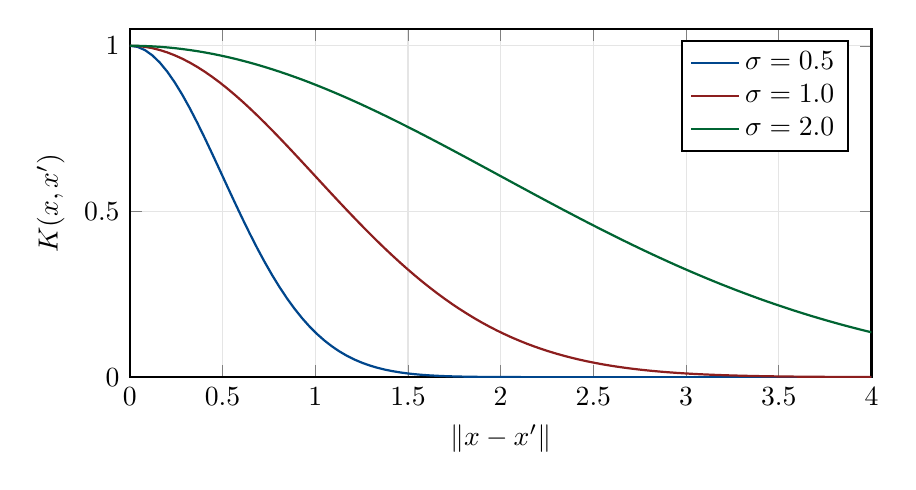
\begin{tikzpicture}
\begin{axis}[
  width=11cm, height=6cm,
  xlabel={$\|x - x'\|$}, ylabel={$K(x,x')$},
  xmin=0, xmax=4, ymin=0, ymax=1.05,
  legend pos=north east,
  grid=major, grid style={gray!20},
  thick
]
\addplot[defblue, domain=0:4, samples=100] {exp(-x^2/(2*0.25))};
\addlegendentry{$\sigma = 0.5$}
\addplot[thmred, domain=0:4, samples=100] {exp(-x^2/(2*1))};
\addlegendentry{$\sigma = 1.0$}
\addplot[exgreen, domain=0:4, samples=100] {exp(-x^2/(2*4))};
\addlegendentry{$\sigma = 2.0$}
\end{axis}
\end{tikzpicture}
\caption{The Gaussian (RBF) kernel $K(x,x') =
\exp(-\norm{x-x'}^2/2\sigma^2)$ as a function of the distance
$\norm{x-x'}$, for three bandwidth values $\sigma$. Smaller $\sigma$
means faster decay: only very nearby points have high similarity.}
\label{rkhs:fig:rbf_kernel}
\end{figure}

% ────────────────────────────
\subsection{Closure Properties}
\label{rkhs:subsec:closure}

Positive definite kernels enjoy useful closure properties that allow us
to build complex kernels from simple ones:

\begin{proposition}[Closure Properties]
\label{rkhs:prop:closure}
If $K_1$ and $K_2$ are p.d.\ kernels and $\alpha > 0$, then the
following are also p.d.\ kernels:
\begin{enumerate}[label=(\roman*)]
  \item $\alpha K_1$ \quad (scaling)
  \item $K_1 + K_2$ \quad (sum)
  \item $K_1 \cdot K_2$ \quad (pointwise product --- Schur product theorem)
  \item $\exp(K_1)$ \quad (exponentiation --- via power series)
\end{enumerate}
\end{proposition}

\begin{proof}
We prove (ii); the others are similar.

Let $c \in \R^m$ be arbitrary. Then:
\[
\sum_{i,j} c_i c_j (K_1 + K_2)(x_i, x_j) = \underbrace{\sum_{i,j} c_i
c_j K_1(x_i, x_j)}_{\geq\, 0} + \underbrace{\sum_{i,j} c_i c_j K_2(x_i,
x_j)}_{\geq\, 0} \;\geq\; 0.
\]
\end{proof}

\begin{insightbox}[Why Closure Matters]
Property (iv) is particularly important: the Gaussian kernel can be
derived from the linear kernel via:
\[
K_{\mathrm{RBF}}(x,x') = \exp\!\bigl(-\norm{x}^2/(2\sigma^2)\bigr) \cdot
\exp\!\bigl(x^\top x'/\sigma^2\bigr) \cdot
\exp\!\bigl(-\norm{x'}^2/(2\sigma^2)\bigr).
\]
Since $K_{\mathrm{lin}}(x,x') = x^\top x'$ is p.d., so is $\exp(x^\top
x'/\sigma^2)$, and the remaining factors are positive scalars depending
on single arguments.
\end{insightbox}


% ══════════════════════════════════════════════════════════════
\section{Feature Maps and the Kernel Trick}
\label{rkhs:sec:feature_maps}
% ══════════════════════════════════════════════════════════════

A kernel $K(x,x')$ implicitly defines a \emph{feature map} that embeds
inputs into a (potentially infinite-dimensional) inner product space
where the kernel value equals the inner product.

\begin{figure}[ht]
\centering
\begin{tikzpicture}[
  >=Stealth,
  point/.style={circle, fill, inner sep=1.5pt},
  every node/.style={font=\small}
]

  % ── Input space X ──
  \begin{scope}
    \draw[thick, defblue, rounded corners=12pt]
      (-1.8,-2.2) rectangle (1.8,2.2);
    \node[defblue, font=\bfseries] at (0,2.6)
      {Input space $\X$};

    % Points
    \node[point, thmred, label={left:$x$}]
      (x) at (-0.4, 0.8) {};
    \node[point, thmred, label={left:$x'$}]
      (xp) at (-0.2,-0.7) {};

    % Kernel value
    \draw[insightorange, thick, <->]
      (x) -- (xp)
      node[midway, right=6pt, insightorange]
      {$K(x,x')$};
  \end{scope}

  % ── Arrow phi ──
  \draw[->, thick, gray!80, line width=1.2pt]
    (2.4, 0) -- node[above, black]
    {$\phi$} (6.6, 0);

  % ── Feature space F ──
  \begin{scope}[xshift=8cm]
    \draw[thick, exgreen, rounded corners=12pt]
      (-0.8,-2.2) rectangle (3.5,2.2);
    \node[exgreen, font=\bfseries] at (1.3,2.6)
      {Feature space $\mathcal{F}$};

    % Origin
    \fill[gray] (0,0) circle (1pt);

    % Mapped points
    \node[point, thmred,
      label={[xshift=3pt]above right:$\phi(x)$}]
      (px) at (0.3, 1.5) {};
    \node[point, thmred,
      label={[xshift=3pt]below right:$\phi(x')$}]
      (pxp) at (1.0, -0.5) {};

    % Vectors from origin
    \draw[->, gray, thick] (0,0) -- (px);
    \draw[->, gray, thick] (0,0) -- (pxp);

    % Angle / inner product
    \draw[insightorange, thick]
      (0.3, -0.18) arc[start angle=-29,
      end angle=75, radius=0.35];
    \node[insightorange, right] at (0.3, 0.5)
      {$\inner{\phi(x)}{\phi(x')}_{\!\mathcal{F}}$};
  \end{scope}

  % ── Equality at bottom ──
  \node[font=\large, insightorange] at (4.4, -2.6)
    {$K(x,\, x')
      \;=\; \inner{\phi(x)}{\phi(x')}_{\mathcal{F}}$};

\end{tikzpicture}
\caption{The feature map idea. A kernel $K$ on the
input space $\X$ (left) corresponds to an inner product
in some feature space $\mathcal{F}$ (right) via a
feature map $\phi$. The only requirement is
$K(x,x') = \inner{\phi(x)}{\phi(x')}_{\mathcal{F}}$
(Definition~\ref{rkhs:def:feature_map}). The kernel trick
exploits this: we compute $K(x,x')$ directly, without
ever forming $\phi(x)$ explicitly.}
\label{rkhs:fig:feature_map_concept}
\end{figure}

% ────────────────────────────
\subsection{From Kernels to Feature Maps}

\begin{definitionbox}[Definition: Feature Map]
\begin{definition}[Feature Map]
\label{rkhs:def:feature_map}
A \textbf{feature map} for a kernel $K$ is a mapping $\phi: \X \to
\mathcal{F}$ into some inner product space $\mathcal{F}$ (the
\textbf{feature space}) such that:
\begin{equation}
\label{rkhs:eq:feature_map}
K(x, x') = \inner{\phi(x)}{\phi(x')}_{\mathcal{F}} \quad \text{for all } x, x' \in \X.
\end{equation}
\end{definition}
\end{definitionbox}

The feature map is \emph{not} unique. For a given kernel, many different
$\phi$ and $\mathcal{F}$ satisfy~\eqref{rkhs:eq:feature_map}. The remarkable
fact is that every p.d.\ kernel \emph{has} such a feature map --- this
is guaranteed by the Moore--Aronszajn theorem
(Section~\ref{rkhs:sec:rkhs_construction}).

% ────────────────────────────
\subsection{The Kernel Trick}
\label{rkhs:subsec:kernel_trick}

\begin{insightbox}[The Kernel Trick --- Core Idea]
Many machine learning algorithms (e.g., SVMs, PCA, ridge regression)
depend on the data \emph{only} through inner products
$\inner{x_i}{x_j}$. If we replace each inner product with a kernel
evaluation $K(x_i, x_j) = \inner{\phi(x_i)}{\phi(x_j)}$, we are
implicitly running the algorithm in the (possibly infinite-dimensional)
feature space $\mathcal{F}$, \textbf{without ever computing $\phi$
explicitly}.
\end{insightbox}

Let us see this concretely.

\begin{examplebox}[Example 7: Kernel Trick for the Polynomial Kernel]
Consider data in $\R^2$: $x = (x_1, x_2)$. We saw in
Example~5 that the quadratic kernel
$K(x,x') = (x^\top x')^2$ can be written as a dot
product in $\R^3$. Defining the feature map:
\[
\phi(x) = \begin{pmatrix} x_1^2 \\
\sqrt{2}\,x_1 x_2 \\ x_2^2
\end{pmatrix} \in \R^3,
\]
we have
$K(x,x') = \phi(x)^\top \phi(x')$.

\textbf{Without the kernel trick}: Map each input to
$\R^3$ via $\phi$, then compute the inner product.
Cost: $O(d^2)$ per pair.

\textbf{With the kernel trick}: Compute $(x^\top x')^2$
directly. Cost: $O(d)$ per pair.

For degree-$p$ polynomial kernels in $\R^d$, the
feature space has dimension $\binom{d+p}{p}$, which
grows explosively. The kernel trick avoids this
entirely.
\end{examplebox}

\begin{figure}[ht]
\centering
\begin{tikzpicture}[scale=0.95]
  % Input space
  \begin{scope}
    \node[above, font=\bfseries] at (0,2.8) {Input space $\R^2$};
    \draw[-{Stealth}, gray] (-2.5,0) -- (2.5,0) node[right, font=\small] {$x_1$};
    \draw[-{Stealth}, gray] (0,-2.1) -- (0,2.2) node[above, font=\small] {$x_2$};

    % Non-linearly separable data: inner ring (class -1)
    \foreach \a in {0,40,...,320} {
      \fill[thmred] ({0.8*cos(\a)},{0.8*sin(\a)}) circle (2pt);
    }
    % Outer ring (class +1)
    \foreach \a in {0,30,...,330} {
      \fill[defblue] ({1.8*cos(\a)},{1.8*sin(\a)}) circle (2pt);
    }
    \node[font=\small, thmred] at (0.2, -0.3) {class $-1$};
    \node[font=\small, defblue] at (0.2, -2.3) {class $+1$};
    \node[font=\footnotesize, gray] at (0, -2.6) {(no linear separator exists)};
  \end{scope}

  % Arrow
  \draw[-{Stealth[length=4mm]}, thick, insightorange] (3.2, 0) -- node[above, font=\small] {$\phi(x) = (x_1^2,\,\sqrt{2}\,x_1 x_2,\,x_2^2)$} (6.3, 0);

  % Feature space (projected view of R^3 showing x_1^2 + x_2^2 axis)
  \begin{scope}[xshift=9.5cm, yshift=-21]
    \node[above, font=\bfseries] at (0,3.5) {Feature space $\R^3$ (projected view)};
    \draw[-{Stealth}, gray] (-2.5,0) -- (2.5,0) node[right, font=\small] {$\sqrt{2}\,x_1 x_2$};
    \draw[-{Stealth}, gray] (0,-0.8) -- (0,3.0) node[above, font=\small] {$x_1^2 + x_2^2$};

    % Inner ring maps to low r^2 values: r=0.8, so x1^2+x2^2 = 0.64
    \foreach \a in {0,40,...,320} {
      \pgfmathsetmacro{\xfeat}{0.8*cos(\a)*0.8*sin(\a)*1.414*1.5}
      \pgfmathsetmacro{\yfeat}{0.64*2.5}
      \fill[thmred] (\xfeat, \yfeat) circle (2pt);
    }
    % Outer ring maps to high r^2 values: r=1.8, so x1^2+x2^2 = 3.24
    \foreach \a in {0,30,...,330} {
      \pgfmathsetmacro{\xfeat}{1.8*cos(\a)*1.8*sin(\a)*1.414*0.7}
      \pgfmathsetmacro{\yfeat}{3.24*0.75}
      \fill[defblue] (\xfeat, \yfeat) circle (2pt);
    }

    % Separating hyperplane (horizontal line between the two bands)
    \draw[exgreen, thick, dashed] (-2.3, 1.95) -- (2.3, 1.95);
    \node[font=\small, exgreen, right] at (1.5, 1.65) {linear separator};
  \end{scope}
\end{tikzpicture}
\caption{The kernel trick in action. Data arranged in
two concentric rings is not linearly separable in the
input space $\R^2$ (left). The feature map
$\phi(x) = (x_1^2,\,\sqrt{2}\,x_1 x_2,\, x_2^2)$
sends points with $\|x\| = r$ to height
$x_1^2 + x_2^2 = r^2$ in $\R^3$, ``lifting'' the
outer ring above the inner ring (right, projected
view). A horizontal hyperplane now separates the
classes. The kernel
$K(x,x') = (x^\top x')^2 = \phi(x)^\top \phi(x')$
lets us work in this feature space without computing
$\phi$ explicitly.}
\label{rkhs:fig:kernel_trick}
\end{figure}


% ══════════════════════════════════════════════════════════════
\section{Constructing the RKHS}
\label{rkhs:sec:rkhs_construction}
% ══════════════════════════════════════════════════════════════

We now construct the RKHS rigorously. The key insight: every positive
definite kernel $K$ generates a \emph{unique} Hilbert space of functions
--- the RKHS $\hk$.

% ────────────────────────────
\subsection{The Canonical Feature Map}
\label{rkhs:subsec:canonical_feature_map}

Among all possible feature maps for $K$, there is a particularly natural one:

\begin{definitionbox}[Definition: Canonical Feature Map]
\begin{definition}[Canonical Feature Map]
\label{rkhs:def:canonical_feature}
For each $x \in \X$, define the function
$K_x: \X \to \R$ by:
\[
K_x(\cdot) := K(\cdot, x).
\]
The mapping $\phi: x \mapsto K_x$ sends each input
point to a \emph{function}. The feature space is a
space of functions.
\end{definition}
\end{definitionbox}

Writing $\phi_x$ for $K_x$, the canonical feature map
is summarized by a single equation:
\begin{equation}
\label{rkhs:eq:canonical_feature}
\boxed{\phi_x(y) \;=\; K(y,\, x)
  \qquad \text{for all } x, y \in \X}
\end{equation}
Every element of the feature space is a function
obtained by ``freezing'' one argument of $K$. All
the key identities follow directly from this:
\begin{itemize}
  \item \textbf{Reproducing property}
    (Section~\ref{rkhs:sec:reproducing_property}):
    $f(x) = \inner{f}{\phi_x}_{\hk}$.
  \item \textbf{Kernel reproduces itself}:
    $K(x,x') = \inner{\phi_x}{\phi_{x'}}_{\hk}$.
\end{itemize}

\textbf{Why is this natural?} Because we can define an
inner product directly:
\[
\inner{K_x}{K_{x'}}_{\hk} := K(x, x').
\]
We then have
$K(x,x') = \inner{\phi_x}{\phi_{x'}}_{\hk}$, exactly
as required by~\eqref{rkhs:eq:feature_map}.

\begin{figure}[ht]
\centering
\begin{tikzpicture}[
  >=Stealth,
  point/.style={circle, fill, inner sep=1.5pt},
  every node/.style={font=\small}
]

  % ── Input space X ──
  \begin{scope}
    \draw[thick, defblue, rounded corners=12pt]
      (-1.8,-2.2) rectangle (1.8,2.2);
    \node[defblue, font=\bfseries] at (0,2.6)
      {Input space $\X$};

    % Points
    \node[point, thmred, label={left:$x$}]
      (x) at (-0.4, 0.8) {};
    \node[point, thmred, label={left:$x'$}]
      (xp) at (-0.2,-0.7) {};

    % Kernel value
    \draw[insightorange, thick, <->]
      (x) -- (xp)
      node[midway, right=6pt, insightorange]
      {$K(x,x')$};
  \end{scope}

  % ── Arrow: canonical feature map ──
  \draw[->, thick, gray!80, line width=1.2pt]
    (2.4, 0) -- node[above, black]
    {$x \;\mapsto\; \phi_x = K(\cdot, x)$}
    (6.6, 0);

  % ── RKHS H_K ──
  \begin{scope}[xshift=8cm]
    \draw[thick, thmred, rounded corners=12pt]
      (-0.8,-2.2) rectangle (3.5,2.2);
    \node[thmred, font=\bfseries] at (1.3,2.6)
      {RKHS $\hk$ (functions)};

    % Origin
    \fill[gray] (0,0) circle (1pt);

    % Mapped points (functions)
    \node[point, thmred,
      label={[xshift=3pt]above right:%
        $\phi_x = K(\cdot,x)$}]
      (px) at (0.3, 1.5) {};
    \node[point, thmred,
      label={[xshift=3pt]below right:%
        $\phi_{x'} = K(\cdot,x')$}]
      (pxp) at (1.0, -0.5) {};

    % Vectors from origin
    \draw[->, gray, thick] (0,0) -- (px);
    \draw[->, gray, thick] (0,0) -- (pxp);

    % Inner product
    \draw[insightorange, thick]
      (0.3, -0.18) arc[start angle=-29,
      end angle=75, radius=0.35];
    \node[insightorange, right] at (0.3, 0.5)
      {$\inner{\phi_x}{\phi_{x'}}_{\!\hk}$};
  \end{scope}

  % ── Equality at bottom ──
  \node[font=\large, insightorange] at (4.4, -2.6)
    {$K(x,\, x')
      \;=\; \inner{\phi_x}{\phi_{x'}}_{\hk}$};

\end{tikzpicture}
\caption{The \emph{canonical} feature map (compare with
the general feature map in Figure~\ref{rkhs:fig:feature_map_concept}).
Here the feature space is specifically the RKHS $\hk$:
each point $x \in \X$ is mapped to the \emph{function}
$\phi_x = K(\cdot, x) \in \hk$. The inner product in
$\hk$ recovers the kernel:
$K(x,x') = \inner{\phi_x}{\phi_{x'}}_{\hk}$.}
\label{rkhs:fig:canonical_feature_map}
\end{figure}

\begin{insightbox}[Multiple Feature Maps and Their
Relationship]
The canonical feature map produces \emph{functions}.
But recall from Section~\ref{rkhs:sec:feature_maps} that
Definition~\ref{rkhs:def:feature_map} only requires
$K(x,x') = \inner{\phi(x)}{\phi(x')}_{\mathcal{F}}$
--- it says nothing about $\phi(x)$ being a function.
Indeed, a kernel can admit other feature maps that
produce \emph{vectors}. Let us compare the two for
the linear and polynomial kernels.

\medskip
\textbf{Linear kernel}
($K(x,x') = x^\top x'$ on $\R^d$).
\begin{enumerate}
  \item \textbf{Explicit feature map}:
    $\phi^{\mathrm{ex}}(x) = x \in \R^d$.
    This maps a point to a \emph{vector} and satisfies
    $K(x,x') = \phi^{\mathrm{ex}}(x)^\top
    \phi^{\mathrm{ex}}(x')$. \checkmark
  \item \textbf{Canonical feature map}
    (Definition~\ref{rkhs:def:canonical_feature}):
    $\phi_x^{\mathrm{can}}(\cdot) = K(\cdot,x)$,
    i.e., the \emph{function}
    $z \mapsto z^\top x$.
    This maps a point to a \emph{linear functional}
    in $\hk$.
\end{enumerate}
The two live in different spaces ($\R^d$ vs.\
$\hk$), but they carry the same information. The
isometric isomorphism $T: \R^d \to \hk$ is the
Riesz map:
\[
T(w) = f_w, \qquad f_w(z) = z^\top w.
\]
Note that $f_w(z) = z^\top w$ matches the kernel form
$K(z,x) = z^\top x$: the canonical feature map
$\phi_x^{\mathrm{can}} = K(\cdot, x)$ is simply
$f_x$.

The RKHS inner product is
$\inner{f_w}{f_v}_{\hk} = w^\top v$, which can be
verified via the reproducing property:
\[
\inner{f_w}{f_v}_{\hk}
= \inner{f_w}{K(\cdot, v)}_{\hk}
= f_w(v) = v^\top w = w^\top v.
\]
$T$ is therefore linear, bijective, and preserves
inner products. Moreover, it intertwines the two
feature maps:
$T \circ \phi^{\mathrm{ex}} = \phi^{\mathrm{can}}$.
\end{insightbox}

\begin{insightbox}[Multiple Feature Maps: Quadratic
Kernel]
The same phenomenon occurs for the quadratic kernel,
but the isomorphism is richer.

\medskip
\textbf{Quadratic kernel}
($K(x,x') = (x^\top x')^2$ on $\R^2$).
\begin{enumerate}
  \item \textbf{Explicit feature map}
    (Example~7):
    $\phi^{\mathrm{ex}}(x) =
    (x_1^2,\, \sqrt{2}\,x_1 x_2,\, x_2^2)^\top
    \in \R^3$.
    This produces a concrete \emph{vector}.
  \item \textbf{Canonical feature map}:
    $\phi_x^{\mathrm{can}}(\cdot) = K(\cdot, x)$,
    i.e., the \emph{function}
    $z \mapsto (z_1 x_1 + z_2 x_2)^2
    = x_1^2 z_1^2 + 2x_1 x_2\, z_1 z_2
    + x_2^2 z_2^2$.
    This produces a function in $\hk$.
\end{enumerate}
The isometric isomorphism $T: \R^3 \to \hk$ maps
a vector to the function whose monomial coefficients
are given by that vector (with the $\sqrt{2}$
rescaling on the cross-term):
\[
T\!\begin{pmatrix} a \\ b \\ c \end{pmatrix}
\;=\; \text{the function } z \mapsto
a\,z_1^2 + \tfrac{b}{\sqrt{2}}\,(2z_1 z_2)
+ c\,z_2^2
\;=\; a\,z_1^2 + \sqrt{2}\,b\, z_1 z_2
+ c\,z_2^2.
\]

\textbf{Verification that
$T \circ \phi^{\mathrm{ex}} = \phi^{\mathrm{can}}$.}
Apply $T$ to $\phi^{\mathrm{ex}}(x) =
(x_1^2,\, \sqrt{2}\,x_1 x_2,\, x_2^2)^\top$:
\[
T\!\bigl(\phi^{\mathrm{ex}}(x)\bigr)(z)
= x_1^2\, z_1^2
+ \tfrac{\sqrt{2}\,x_1 x_2}{\sqrt{2}}\,(2z_1 z_2)
+ x_2^2\, z_2^2
= x_1^2 z_1^2 + 2x_1 x_2\, z_1 z_2
+ x_2^2 z_2^2
= (z^\top x)^2 = \phi_x^{\mathrm{can}}(z).
\quad\checkmark
\]

\textbf{Verification that $\inner{u}{v}_{\R^3} =
\inner{Tu}{Tv}_{\hk}$.} It suffices to check that $T$
maps the standard basis $\{e_1, e_2, e_3\}$ of $\R^3$
to an orthonormal set in $\hk$. The images are:
\[
Te_1 = z_1^2, \qquad
Te_2 = \sqrt{2}\,z_1 z_2, \qquad
Te_3 = z_2^2.
\]
To compute RKHS inner products, we express each $Te_i$
as a linear combination of canonical feature maps
$K(\cdot, x) = (z^\top x)^2$, then use the fundamental
identity
$\inner{K(\cdot,x)}{K(\cdot,x')}_{\hk} = K(x,x')
= (x^\top x')^2$.

Writing $\mat{e}_1 = (1,0)^\top$ and
$\mat{e}_2 = (0,1)^\top$ for the standard basis of
$\R^2$, we have
$K(\cdot, \mat{e}_1) = z_1^2$ and
$K(\cdot, \mat{e}_2) = z_2^2$, so:
\[
Te_1 = K(\cdot, \mat{e}_1), \qquad
Te_3 = K(\cdot, \mat{e}_2).
\]
For the cross-term, expanding
$K(\cdot, \mat{e}_1{+}\mat{e}_2) = (z_1{+}z_2)^2
= z_1^2 + 2z_1 z_2 + z_2^2$ gives:
\[
Te_2 = \sqrt{2}\,z_1 z_2
= \tfrac{\sqrt{2}}{2}\bigl[
K(\cdot, \mat{e}_1{+}\mat{e}_2)
- K(\cdot, \mat{e}_1) - K(\cdot, \mat{e}_2)\bigr].
\]
Now all inner products reduce to evaluating
$(x^\top x')^2$. The diagonal terms:
\begin{align*}
\inner{Te_1}{Te_1}_{\hk}
&= K(\mat{e}_1, \mat{e}_1) = 1, \\
\inner{Te_3}{Te_3}_{\hk}
&= K(\mat{e}_2, \mat{e}_2) = 1.
\end{align*}
For $\inner{Te_2}{Te_2}_{\hk}$, we use bilinearity
with $s = \mat{e}_1{+}\mat{e}_2$ and the needed
kernel values $K(s,s) = 4$,
$K(s,\mat{e}_1) = K(s,\mat{e}_2) = 1$,
$K(\mat{e}_1,\mat{e}_2) = 0$:
\begin{align*}
\inner{Te_2}{Te_2}_{\hk}
&= \tfrac{1}{2}\bigl[
  K(s,s) - 2K(s,\mat{e}_1) - 2K(s,\mat{e}_2)
  + K(\mat{e}_1,\mat{e}_1)
  + 2K(\mat{e}_1,\mat{e}_2)
  + K(\mat{e}_2,\mat{e}_2)
\bigr] \\
&= \tfrac{1}{2}[4 - 2 - 2 + 1 + 0 + 1] = 1.
\end{align*}
The off-diagonal terms vanish similarly (e.g.,
$\inner{Te_1}{Te_2}_{\hk}
= \frac{\sqrt{2}}{2}[K(\mat{e}_1, s)
- K(\mat{e}_1, \mat{e}_1)
- K(\mat{e}_1, \mat{e}_2)]
= \frac{\sqrt{2}}{2}[1 - 1 - 0] = 0$).
Therefore $\{Te_1, Te_2, Te_3\}$ is orthonormal in
$\hk$, and by bilinearity:
\[
\inner{Tu}{Tv}_{\hk}
= \sum_{i,j} u_i v_j
  \underbrace{\inner{Te_i}{Te_j}_{\hk}}_{%
    =\,\delta_{ij}}
= \sum_i u_i v_i
= \inner{u}{v}_{\R^3}.
\quad\checkmark
\]
\end{insightbox}

\begin{insightbox}[The Canonical Feature Map is Universal]
\textbf{The general principle.} Every valid feature
map factors through the canonical one via an isometry.
The canonical feature map is ``universal'': all others
are concrete realizations of it.

\textbf{Why does this matter?} When $\hk$ is
finite-dimensional (linear or polynomial kernel), we
can choose the explicit vector representation
$\phi^{\mathrm{ex}}$ and never think about functions
--- the isomorphism loses nothing. When $\hk$ is
infinite-dimensional (Gaussian kernel), no finite
vector representation exists, and the canonical
feature map into a space of functions is the only
option.
\end{insightbox}

% ────────────────────────────
\subsection{Building the Space Step by Step}
\label{rkhs:subsec:building_space}

The canonical feature map tells us \emph{what} the
RKHS should contain (the functions $K(\cdot, x)$ and
their linear combinations), but it does not yet give
us a complete Hilbert space with a well-defined inner
product. The goal of this subsection is to construct
$\hk$ rigorously from $K$ alone, culminating in the
Moore--Aronszajn theorem which guarantees that this
construction yields a \textbf{unique} RKHS. The
construction proceeds in four stages:

\textbf{Step 1: Start with kernel sections.} For each $x \in \X$, we
have the function $K_x = K(\cdot, x)$ in our space.

\textbf{Step 2: Take finite linear combinations.} Define:
\[
\hilb_0 := \Bigl\{ f = \sum_{i=1}^m \alpha_i\, K_{x_i} \;\Big|\; m \in
\N,\; \alpha_i \in \R,\; x_i \in \X \Bigr\}.
\]
These are functions of the form $f(\cdot) = \sum_{i=1}^m \alpha_i
K(\cdot, x_i)$.

\textbf{Step 3: Define the inner product.} For $f = \sum_i \alpha_i
K_{x_i}$ and $g = \sum_j \beta_j K_{x_j'}$:
\begin{equation}
\label{rkhs:eq:inner_product_h0}
\inner{f}{g}_{\hilb_0} := \sum_{i,j} \alpha_i \beta_j\, K(x_i, x_j').
\end{equation}

\begin{lemma}[Well-definedness]
\label{rkhs:lem:well_defined}
The inner product~\eqref{rkhs:eq:inner_product_h0} is well-defined (i.e., it
does not depend on the particular representation of $f$ and $g$) and
satisfies all inner product axioms.
\end{lemma}

\begin{proof}
\textbf{Well-definedness.} Suppose $f$ has two
representations:
$f = \sum_{i=1}^m \alpha_i K_{x_i}
   = \sum_{k=1}^{m'} \gamma_k K_{y_k}$.
We must show that $\inner{f}{g}$ gives the same value
regardless of which representation of $f$ we use, for
any $g = \sum_{j=1}^n \beta_j K_{x_j'} \in \hilb_0$.

It suffices to show: if
$h = \sum_{i=1}^m \alpha_i K_{x_i}
   - \sum_{k=1}^{m'} \gamma_k K_{y_k} = 0$
as a function (i.e., $h(x) = 0$ for all $x \in \X$),
then $\inner{h}{g} = 0$ for all $g \in \hilb_0$.
Indeed, once this is established, the two
representations of $f$ give:
\[
\sum_{i,j} \alpha_i \beta_j K(x_i, x_j')
- \sum_{k,j} \gamma_k \beta_j K(y_k, x_j')
= \inner{h}{g} = 0.
\]

To prove $\inner{h}{g} = 0$, we first check it for
a single kernel section $g = K_{x'}$:
\[
\inner{h}{K_{x'}}
\;=\; \inner*{\sum_i \alpha_i K_{x_i}
  - \sum_k \gamma_k K_{y_k},\; K_{x'}}
\;=\; \sum_i \alpha_i K(x_i, x')
  - \sum_k \gamma_k K(y_k, x')
\;=\; h(x').
\]
The first equality applies
formula~\eqref{rkhs:eq:inner_product_h0} to each term.
The second equality uses the definition of $h$ as
a function: $h(x') = \sum_i \alpha_i K(x', x_i)
- \sum_k \gamma_k K(x', y_k)$, together with the
symmetry $K(x_i, x') = K(x', x_i)$. Since $h = 0$
as a function, $h(x') = 0$ for every $x' \in \X$,
so $\inner{h}{K_{x'}} = 0$ for every $x'$.

For a general $g = \sum_j \beta_j K_{x_j'}$, we
conclude by linearity:
\[
\inner{h}{g}
= \sum_j \beta_j \inner{h}{K_{x_j'}}
= \sum_j \beta_j \cdot 0 = 0.
\qquad\checkmark
\]

\medskip
\textbf{Positive semi-definiteness}
($\inner{f}{f} \geq 0$) follows directly from the
positive definiteness of $K$:
$\inner{f}{f} = \sum_{i,j} \alpha_i \alpha_j
K(x_i, x_j) \geq 0$.

\medskip
\textbf{Positive definiteness}
($\inner{f}{f} = 0 \implies f = 0$): note that
$\inner{f}{K_x} = f(x)$ by the computation above.
So if $\inner{f}{f} = 0$, then by Cauchy--Schwarz
$|f(x)|^2 = |\inner{f}{K_x}|^2
\leq \inner{f}{f}\,\inner{K_x}{K_x} = 0$
for all $x$, giving $f \equiv 0$.
\end{proof}

\textbf{Step 4: Complete the space.} The space $\hilb_0$ with this inner
product may not be complete. We form the \textbf{completion} $\hk =
\overline{\hilb_0}$ by including all limits of Cauchy sequences from
$\hilb_0$. The resulting space $\hk$ is a Hilbert space.

\begin{theorembox}[Theorem: Moore--Aronszajn]
\begin{theorem}[Moore--Aronszajn Theorem]
\label{rkhs:thm:moore_aronszajn}
For every positive definite kernel $K$ on $\X \times \X$, there exists a
\textbf{unique} Hilbert space $\hk$ of functions $f: \X \to \R$ such
that:
\begin{enumerate}[label=(\roman*)]
  \item $K(\cdot, x) \in \hk$ for every $x \in \X$.
  \item $f(x) = \inner{f}{K(\cdot, x)}_{\hk}$ for every $f \in \hk$ and
  every $x \in \X$.
\end{enumerate}
This space $\hk$ is called the \textbf{Reproducing Kernel Hilbert Space} of $K$.
\end{theorem}
\end{theorembox}

Property (ii) is the \emph{reproducing property} --- the defining
characteristic of RKHS. We develop it carefully in the next section.


% ══════════════════════════════════════════════════════════════
\section{The Reproducing Property}
\label{rkhs:sec:reproducing_property}
% ══════════════════════════════════════════════════════════════

The reproducing property is the most important and distinctive feature
of an RKHS. Let us state it carefully, prove it, and explore its
consequences.

% ────────────────────────────
\subsection{Statement and Proof}

\begin{theorembox}[The Reproducing Property]
\begin{proposition}[Reproducing Property]
\label{rkhs:prop:reproducing}
In the RKHS $\hk$ constructed above, for every $f \in \hk$ and every $x \in \X$:
\begin{equation}
\label{rkhs:eq:reproducing}
\boxed{f(x) = \inner{f}{K(\cdot, x)}_{\hk}}
\end{equation}
That is: \textbf{evaluation at $x$} equals \textbf{inner product with
$K(\cdot, x)$}.
\end{proposition}
\end{theorembox}

\begin{proof}
\textbf{Step 1:} For ``kernel sections'', i.e., functions of the form
$K_y = K(\cdot, y)$:
\[
\inner{K_y}{K_x}_{\hk} = K(y, x) = K_y(x).
\]
The first equality is by definition of the inner
product~\eqref{rkhs:eq:inner_product_h0}. The second is by definition of
$K_y$. So the reproducing property holds for $f = K_y$.

\textbf{Step 2:} For finite linear combinations
$f = \sum_{i=1}^m \alpha_i K_{x_i} \in \hilb_0$, we
use the linearity of the inner product (in the first
argument) and the result of Step~1:
\begin{align*}
\inner{f}{K_x}_{\hk}
&= \left\langle \sum_{i=1}^m \alpha_i K_{x_i},\;
   K_x \right\rangle_{\!\hk}
   && \text{(replacing $f$ by its definition
   in $\hilb_0$)} \\
&= \sum_{i=1}^m \alpha_i
   \inner{K_{x_i}}{K_x}_{\hk}
   && \text{(linearity)} \\
&= \sum_{i=1}^m \alpha_i\, K(x_i, x)
   && \text{(Step 1)} \\
&= \sum_{i=1}^m \alpha_i\, K(x, x_i)
   && \text{(symmetry of $K$)} \\
&= f(x).
   && \text{(definition of
   $f(x) = \textstyle\sum_i \alpha_i K_{x_i}(x)
   = \textstyle\sum_i \alpha_i K(x, x_i)$)}
\end{align*}

\textbf{Step 3:} For general $f \in \hk$. Since $\hk$
is the completion of $\hilb_0$, there exists a
sequence $(f_n)$ in $\hilb_0$ with
$f_n \to f$ in $\hk$-norm, i.e.,
$\norm{f_n - f}_{\hk} \to 0$. By Step~2,
$f_n(x) = \inner{f_n}{K_x}_{\hk}$ for each $n$.
We pass to the limit on both sides.

\emph{Right-hand side:}
$\inner{f_n}{K_x}_{\hk} \to \inner{f}{K_x}_{\hk}$.
This follows from the \textbf{Cauchy--Schwarz
inequality} $|\inner{u}{v}| \leq \norm{u}\,\norm{v}$,
which holds in any inner product space. Applying it
with $u = f_n - f$ and $v = K_x$:
\[
\bigl|\inner{f_n}{K_x}_{\hk}
  - \inner{f}{K_x}_{\hk}\bigr|
= \bigl|\inner{f_n - f}{K_x}_{\hk}\bigr|
\leq \underbrace{\norm{f_n - f}_{\hk}}_{\to\, 0}
  \cdot\; \norm{K_x}_{\hk}
\;\xrightarrow{n \to \infty}\; 0.
\]

\emph{Left-hand side:}
$f_n(x) \to f(x)$. Since each $f_n - f_m$ lies in
$\hilb_0$, Step~2 gives
$(f_n - f_m)(x) = \inner{f_n - f_m}{K_x}_{\hk}$,
so by Cauchy--Schwarz:
\[
|f_n(x) - f_m(x)|
= \bigl|\inner{f_n - f_m}{K_x}_{\hk}\bigr|
\leq \norm{f_n - f_m}_{\hk} \cdot \norm{K_x}_{\hk}.
\]
Since $(f_n)$ is Cauchy in $\hk$-norm,
$(f_n(x))$ is Cauchy in $\R$, hence converges.
We define $f(x) := \lim_n f_n(x)$ (this is how
functions in the completion $\hk$ are evaluated
pointwise).

Combining: $f(x) = \lim_{n} f_n(x)
= \lim_{n} \inner{f_n}{K_x}_{\hk}
= \inner{f}{K_x}_{\hk}$.
\end{proof}

\textbf{Reading the reproducing property.} There are three equivalent
ways to read equation~\eqref{rkhs:eq:reproducing}:
\begin{enumerate}[label=(\alph*)]
  \item \textbf{Evaluation as inner product}: To evaluate $f$ at $x$,
  take the inner product with $K(\cdot, x)$.
  \item \textbf{$K(\cdot, x)$ as ``representer of evaluation''}: The
  function $K(\cdot, x)$ ``represents'' the evaluation functional
  $\delta_x: f \mapsto f(x)$.
  \item \textbf{Kernel reproduces itself}: If you take $f = K(\cdot, y)$
  in the reproducing property
  $f(x) = \langle f, K(\cdot, x) \rangle_{\mathcal{H}_K}$
  you get $K(y,x) = \inner{K(\cdot,y)}{K(\cdot,x)}_{\hk}$, i.e., the
  kernel ``reproduces'' itself through the inner product. This is the
  origin of the name.
\end{enumerate}

\begin{figure}[ht]
\centering
\begin{tikzpicture}[
  >=Stealth,
  point/.style={circle, fill, inner sep=1.5pt},
  every node/.style={font=\small}
]

  % ── Input space X ──
  \begin{scope}
    \draw[thick, defblue, rounded corners=12pt]
      (-1.8,-2.2) rectangle (1.8,2.2);
    \node[defblue, font=\bfseries] at (0,2.6)
      {Input space $\X$};

    % Point x
    \node[point, thmred, label={left:$x$}]
      (x) at (-0.3, 0.4) {};

    % Show f(x) as the output
    \node[insightorange, font=\normalsize]
      at (0.0, -1.4)
      {$f(x) = \;?$};
  \end{scope}

  % ── Arrow: canonical feature map ──
  \draw[->, thick, gray!80, line width=1.2pt]
    (2.4, 0) -- node[above, black]
    {$x \;\mapsto\; \phi_x = K(\cdot, x)$}
    (6.6, 0);

  % ── RKHS H_K ──
  \begin{scope}[xshift=8.2cm]
    \draw[thick, thmred, rounded corners=12pt]
      (-1.2,-2.2) rectangle (5.5,2.2);
    \node[thmred, font=\bfseries] at (1.4,2.6)
      {RKHS $\hk$};

    % Origin
    \fill[gray] (0,0) circle (1pt);

    % K(.,x) vector — pointing right and slightly up
    \node[point, thmred,
      label={[thmred, xshift=-4pt, yshift=3pt]below right:%
        $\phi_x = K(\cdot,x)$}]
      (kx) at (3.0, 0.6) {};
    \draw[->, thmred, thick] (0,0) -- (kx);

    % f vector — pointing up-right, clearly not
    % orthogonal to K(.,x)
    \node[point, defblue,
      label={[defblue, xshift=-1pt, yshift=-5pt] above left:$f$}]
      (f) at (1.8, 1.8) {};
    \draw[->, defblue, thick] (0,0) -- (f);

    % Projection of f onto K(.,x) direction
    % proj = (<f,kx>/|kx|^2) * kx
    % kx direction ~ (3.0, 0.6), f ~ (1.8, 1.8)
    % dot = 5.4+1.08 = 6.48, |kx|^2 = 9+0.36 = 9.36
    % t = 6.48/9.36 ~ 0.692
    % proj ~ (2.08, 0.415)
    \coordinate (proj) at (2.08, 0.415);
    \draw[dashed, gray] (f) -- (proj);
    \fill[insightorange] (proj) circle (1.5pt);

    % Right angle mark at projection
    % perpendicular direction ~ (-0.6, 3.0) normalised
    % short segments for the right angle
    \draw[gray, thin]
      ($(proj) + (-0.05, 0.13)$) --
      ($(proj) + (0.12, 0.17)$) --
      ($(proj) + (0.14, 0.04)$);

    % Inner product annotation
  \draw[insightorange, thick, decorate, 
    decoration={brace, amplitude=4pt, mirror, raise=2pt}] 
    (0,0) -- (proj)
    node[midway, sloped, below=6pt, insightorange, font=\normalsize] 
    {$\langle f, \phi_x \rangle_{\mathcal{H}_K} = f(x)$};

  \end{scope}

\end{tikzpicture}
\caption{Geometric view of the reproducing property
(compare with
Figure~\ref{rkhs:fig:canonical_feature_map}).
In the RKHS $\hk$, both $f$ and
$\phi_x = K(\cdot, x)$ live as ``vectors.'' The
reproducing property says that \emph{evaluating} $f$
at a point $x \in \X$ equals the \emph{inner product}
$\inner{f}{\phi_x}_{\hk}$: geometrically, $f(x)$ is
the (scaled\protect\footnotemark) projection of $f$
onto the direction of $K(\cdot, x)$.}
\label{rkhs:fig:reproducing_property}
\end{figure}
\footnotetext{The \emph{orthogonal projection} of $f$
onto the direction of $\phi_x$ has length
$|\inner{f}{\phi_x}|/\norm{\phi_x}
= |f(x)|/\sqrt{K(x,x)}$, whereas
$f(x) = \inner{f}{\phi_x}$ itself equals this
length \emph{times} $\norm{\phi_x} = \sqrt{K(x,x)}$.
The two coincide only when $K(x,x) = 1$ (e.g., for
the Gaussian kernel), so ``scaled'' accounts for the
general case.}

% ────────────────────────────
\subsection{Continuity of Evaluation}

The reproducing property has a powerful consequence.
In machine learning, we care about predicting
$f(x)$ at specific points (data points, test points).
This requires point evaluation to be a
\emph{continuous} operation: small changes in $f$
(in the RKHS norm) should produce small changes in
$f(x)$. The reproducing property guarantees this.

\begin{theorembox}[Continuous Point Evaluation]
\begin{proposition}[Evaluation is Continuous]
\label{rkhs:prop:eval_continuous}
In an RKHS, point evaluation is a bounded (continuous)
linear functional. Specifically:
\begin{equation}
\label{rkhs:eq:eval_bound}
|f(x)| \leq \sqrt{K(x,x)} \cdot \norm{f}_{\hk}
\quad \text{for all } f \in \hk,\; x \in \X.
\end{equation}
\end{proposition}
\end{theorembox}

\begin{proof}
By the reproducing property and Cauchy--Schwarz:
\begin{align*}
|f(x)|
&= |\inner{f}{K(\cdot,x)}_{\hk}|
  && \text{(reproducing property)} \\
&\leq \norm{f}_{\hk} \cdot
  \norm{K(\cdot,x)}_{\hk}
  && \text{(Cauchy--Schwarz)} \\
&= \norm{f}_{\hk} \cdot
  \sqrt{\inner{K(\cdot,x)}{K(\cdot,x)}_{\hk}}
  && \text{(definition of norm)} \\
&= \norm{f}_{\hk} \cdot \sqrt{K(x,x)}.
  && \text{(reproducing property again)}
\end{align*}
\end{proof}

\begin{insightbox}[Why This Matters: RKHS vs.\ $L^2$]
Not all function spaces enjoy this property.
In the space $L^2([0,1])$, two functions $f$ and $g$
are considered \emph{the same} if they differ only on
a set of measure zero (e.g., at a single point). This
means $f$ and $g$ can have different values at a given
$x$, yet $\norm{f - g}_{L^2} = 0$: point evaluation
is not a continuous operation with respect to the
$L^2$ norm. In formal terms, elements of $L^2$ are
\emph{equivalence classes} of functions, not functions
in the classical sense, so ``$f(x)$'' is ambiguous.

In an RKHS, Proposition~\ref{rkhs:prop:eval_continuous}
rules this out: if $\norm{f - g}_{\hk} = 0$, then
$|f(x) - g(x)| \leq \sqrt{K(x,x)}
\cdot \norm{f - g}_{\hk} = 0$ for every $x$, so
$f$ and $g$ agree \emph{everywhere}. Point evaluation
is well-defined and continuous. This is what makes
RKHS the right setting for regression and
interpolation, where we care about function values
at specific data points.

Inequality~\eqref{rkhs:eq:eval_bound} also shows that if
$\norm{f}_{\hk}$ is small (the function is
``simple''), then $|f(x)|$ is bounded. This is the
mathematical basis for using $\norm{f}_{\hk}^2$ as a
regularizer.
\end{insightbox}

% ────────────────────────────
\subsection{Concrete Numerical Example}

\begin{examplebox}[Example 8: Reproducing Property in Action]
Let $\X = \{a, b\}$ (a two-point domain) with kernel:
\[
K(a,a) = 2, \quad K(a,b) = K(b,a) = 1, \quad K(b,b) = 2.
\]
The Gram matrix $\mat{K} = \begin{psmallmatrix} 2 & 1 \\ 1 & 2
\end{psmallmatrix}$ is PSD (eigenvalues $3$ and $1$). \checkmark

The RKHS $\hk$ consists of functions $f: \{a,b\} \to \R$, which are just
pairs $(f(a), f(b)) \in \R^2$.

The kernel sections are:
\[
K_a = K(\cdot, a): \quad K_a(a) = 2,\; K_a(b) = 1, \qquad K_b = K(\cdot,
b): \quad K_b(a) = 1,\; K_b(b) = 2.
\]

Consider $f = 3K_a - K_b$, i.e., $f(a) = 3 \cdot 2 - 1 \cdot 1 = 5$ and
$f(b) = 3 \cdot 1 - 1 \cdot 2 = 1$.

\textbf{Verify the reproducing property at $x = a$}:
\[
\inner{f}{K_a}_{\hk} = \inner{3K_a - K_b}{K_a}_{\hk} =
3\underbrace{K(a,a)}_{=2} - \underbrace{K(b,a)}_{=1} = 6 - 1 = 5 = f(a).
\quad\checkmark
\]

\textbf{Verify at $x = b$}:
\[
\inner{f}{K_b}_{\hk} = 3\underbrace{K(a,b)}_{=1} -
\underbrace{K(b,b)}_{=2} = 3 - 2 = 1 = f(b). \quad\checkmark
\]

\textbf{Compute the RKHS norm}:
\[
\norm{f}_{\hk}^2 = \inner{3K_a - K_b}{3K_a - K_b}_{\hk} = 9K(a,a) -
3K(a,b) - 3K(b,a) + K(b,b) = 18 - 3 - 3 + 2 = 14.
\]

\textbf{Remark on ``similarity.''}
Note that $K(a,b) = 1$ while $K(a,a) = K(b,b) = 2$:
the off-diagonal values are smaller than the diagonal
ones, but they are not zero. In many presentations,
kernels are described as ``similarity measures.''
This example shows the picture is more nuanced:
$K(x,x')$ is an \emph{inner product} in the feature
space, and while inner products do encode geometric
relationships (through angles and projections), they
are not necessarily bounded between $0$ and $1$ or
interpretable as a ``degree of similarity'' in the
everyday sense. The Gaussian kernel, with
$K(x,x) = 1$ for all $x$ and
$0 < K(x,x') \leq 1$, is the exception that
happens to behave like a similarity measure.
\end{examplebox}


% ══════════════════════════════════════════════════════════════
\section{The Representer Theorem}
\label{rkhs:sec:representer}
% ══════════════════════════════════════════════════════════════

The Representer Theorem is the practical workhorse of kernel methods. It
says: \emph{when you optimize over the entire (infinite-dimensional)
RKHS with an RKHS-norm regularizer, the solution is always a finite
linear combination of kernel evaluations at the data points.}

% ────────────────────────────
\subsection{Statement}

\begin{theorembox}[Theorem: Representer Theorem (Sch\"olkopf et al., 2001)]
\begin{theorem}[Representer Theorem]
\label{rkhs:thm:representer}
Let $\hk$ be an RKHS with kernel $K$, and let $x_1, \ldots, x_n \in \X$
be data points. Consider any optimization problem of the form:
\begin{equation}
\label{rkhs:eq:representer_problem}
\min_{f \in \hk}\;
\underbrace{\sum_{i=1}^n \ell(f(x_i), y_i)}_{\text{data-dependent loss}}
+ \underbrace{
  \lambda \norm{f}_{\hk}^2}_{\text{complexity penalty}\footnote{
    The RKHS norm $\norm{f}_{\hk}^2$ quantifies function complexity:
    by Mercer's theorem (Appendix~\ref{rkhs:sec:mercer}),
    $\norm{f}_{\hk}^2 = \sum_k a_k^2/\lambda_k$, where $\lambda_k$
    are the kernel eigenvalues. Components along high-frequency
    eigenfunctions (small $\lambda_k$) are penalized heavily,
    making $\norm{f}_{\hk}$ a measure of ``roughness'' or oscillation.}}
\end{equation}
where $\ell: \R \times \R \to \R$ is any loss function and $\lambda >
0$. Then the minimizer $f^*$ has the form:
\begin{equation}
\label{rkhs:eq:representer_solution}
\boxed{f^*(x) = \sum_{i=1}^n \alpha_i\, K(x, x_i)} \quad \text{for some } \alpha_1, \ldots, \alpha_n \in \R.
\end{equation}
\end{theorem}
\end{theorembox}

\textbf{Interpretation.} Despite searching over the entire
infinite-dimensional space $\hk$, the optimal function is determined by
just $n$ real numbers $\alpha_1, \ldots, \alpha_n$.

% ────────────────────────────
\subsection{Complete Proof}

\begin{proof}
The proof uses the orthogonal decomposition from Theorem~\ref{rkhs:thm:ortho_decomp}.

\textbf{Step 1: Define the subspace.} Let $M = \spn\{K(\cdot, x_1),
\ldots, K(\cdot, x_n)\} \subseteq \hk$. This is a finite-dimensional
(hence closed) subspace.

\textbf{Step 2: Decompose.} Any $f \in \hk$ decomposes uniquely as $f =
f_\parallel + f_\perp$ with $f_\parallel \in M$ and $f_\perp \in
M^\perp$. Concretely:
\[
f_\parallel = \sum_{i=1}^n \alpha_i K(\cdot, x_i), \qquad
\inner{f_\perp}{K(\cdot, x_j)}_{\hk} = 0 \text{ for all } j.
\]

\textbf{Step 3: $f_\perp$ is invisible to the loss.} By the reproducing
property:
\[
f(x_j) = \inner{f}{K(\cdot, x_j)}_{\hk} = \inner{f_\parallel}{K(\cdot,
x_j)} + \underbrace{\inner{f_\perp}{K(\cdot, x_j)}}_{= 0} =
f_\parallel(x_j).
\]
So $f(x_j) = f_\parallel(x_j)$ for all $j = 1, \ldots, n$. The loss
$\sum_i \ell(f(x_i), y_i)$ depends only on $f_\parallel$.

\textbf{Step 4: $f_\perp$ only increases the regularizer.} By the
Pythagorean theorem:
\[
\norm{f}_{\hk}^2 = \norm{f_\parallel}_{\hk}^2 + \norm{f_\perp}_{\hk}^2
\geq \norm{f_\parallel}_{\hk}^2,
\]
with equality if and only if $f_\perp = 0$.

\textbf{Step 5: Conclude.} The objective is:
\[
J(f) = \underbrace{\sum_{i=1}^n \ell(f(x_i), y_i)}_{\text{depends only
on } f_\parallel} + \lambda\bigl(\norm{f_\parallel}^2 +
\norm{f_\perp}^2\bigr).
\]
Since $\norm{f_\perp}^2 \geq 0$, setting $f_\perp = 0$ can only decrease
(or maintain) the objective. Therefore, the minimizer satisfies $f^* =
f_\parallel^* \in M$, i.e.:
\[
f^*(x) = \sum_{i=1}^n \alpha_i K(x, x_i). \qedhere
\]
\end{proof}

\begin{figure}[ht]
\centering
\begin{tikzpicture}[scale=1.5]
  % The large space H_K
  \draw[rounded corners=8pt, thick, gray] (-4.5,-1) rectangle (5,2.7);
  \node[gray, font=\large] at (3.5, 2.3) {$\hk$};

  % Subspace M
  \fill[blue!6] (-3,-0.8) -- (3,-0.8) -- (3,0.8) -- (-3,0.8) -- cycle;
  \draw[defblue, thick] (-3,0) -- (3,0);
  \node[defblue, font=\small] at (-2.5, 0.2)
  {$M = \spn\{K(\cdot,x_1),\ldots,K(\cdot,x_n)\}$};

  % An arbitrary f
  \draw[-{Stealth[length=3mm]}, thick] (0,0) -- (1.5, 2.2) node[above right] {$f$};

  % Its projection
  \draw[-{Stealth[length=3mm]}, defblue, thick] (0,0) -- (1.5, 0) node[below, font=\small] {$f_\parallel = \sum \alpha_i K(\cdot, x_i)$};

  % Perp component
  \draw[-{Stealth[length=3mm]}, thmred, thick, dashed] (1.5,0) -- (1.5, 2.2);
  \node[thmred, font=\small, right] at (1.6, 1.1) {$f_\perp$};

  % Right angle marker
  \draw[thick] (1.3, 0) -- (1.3, 0.2) -- (1.5, 0.2);

  % Labels
  \node[font=\small] at (-1, -0.7) {Loss sees only $f_\parallel(x_i) = f(x_i)$};
  \node[font=\small, thmred] at (3, -0.7) {$f_\perp$ only adds to $\norm{f}^2_{\hk}$};

  % Origin
  \fill (0,0) circle (1pt);
\end{tikzpicture}
\caption{Geometric intuition for the Representer Theorem. The loss
function sees only $f_\parallel$ (the projection onto the span of kernel
sections at data points). The perpendicular component $f_\perp$ is
invisible to the loss but increases the regularizer. Therefore, the
optimal $f^*$ has $f_\perp = 0$.}
\label{rkhs:fig:representer}
\end{figure}

% ────────────────────────────
\subsection{Kernelization: From Infinite to Finite Dimensions}

The Representer Theorem reduces the infinite-dimensional
optimization~\eqref{rkhs:eq:representer_problem} to a finite-dimensional
problem over $\vect{\alpha} = (\alpha_1, \ldots, \alpha_n)^\top \in
\R^n$. Let us work out the details.

\textbf{Loss term.} Substituting $f^*(x) = \sum_j \alpha_j K(x, x_j)$:
\[
f^*(x_i) = \sum_{j=1}^n \alpha_j K(x_i, x_j) = (\mat{K}\vect{\alpha})_i,
\]
where $\mat{K}$ is the $n \times n$ Gram matrix with $\mat{K}_{ij} =
K(x_i, x_j)$.

\textbf{Regularizer.} Using the reproducing property twice:

\begin{align*}
\norm{f^*}_{\hk}^2 &=
\left\langle \sum_{i=1}^n \alpha_i K(\cdot, x_i),\;
\sum_{j=1}^n \alpha_j K(\cdot, x_j) \right\rangle_{\hk} \nonumber \\
&= \sum_{i,j} \alpha_i \alpha_j
\underbrace{\left\langle K(\cdot, x_i), K(\cdot, x_j)
\right\rangle_{\hk}}_{= K(x_i, x_j)
\text{ (reproducing property)}} \nonumber \\
&= \sum_{i,j} \alpha_i \alpha_j K(x_i, x_j) \;=\;
\vect{\alpha}^\top \mat{K}\, \vect{\alpha}. \label{rkhs:eq:rkhs_norm_alpha}
\end{align*}

\textbf{Full kernelized problem:}
\begin{equation}
\label{rkhs:eq:kernelized}
\boxed{\min_{\vect{\alpha} \in \R^n}\; \sum_{i=1}^n \ell\bigl((\mat{K}\vect{\alpha})_i,\; y_i\bigr) + \lambda\, \vect{\alpha}^\top \mat{K}\, \vect{\alpha}}
\end{equation}

This is a standard finite-dimensional optimization problem involving
only the computable Gram matrix $\mat{K}$.

\begin{examplebox}[Example 9: Kernel Ridge Regression]
With squared loss $\ell(p, y) = (p - y)^2$, the kernelized
problem~\eqref{rkhs:eq:kernelized} becomes:
\[
\min_{\vect{\alpha}} \norm{\mat{K}\vect{\alpha} - \mat{y}}^2 + \lambda\,
\vect{\alpha}^\top \mat{K} \vect{\alpha}.
\]
Taking the gradient and setting it to zero:
\begin{align*}
2\mat{K}(\mat{K}\vect{\alpha} - \mat{y}) + 2\lambda\mat{K}\vect{\alpha} &= 0 \\
\mat{K}^2\vect{\alpha} + \lambda\mat{K}\vect{\alpha} &= \mat{K}\mat{y} \\
\mat{K}(\mat{K} + \lambda \mat{I})\vect{\alpha} &= \mat{K}\mat{y}.
\end{align*}
Since $\mat{K}$ is PSD and $\lambda > 0$, we get $(\mat{K} +
\lambda\mat{I})$ is invertible, and the solution is:
\[
\vect{\alpha}^* = (\mat{K} + \lambda\mat{I})^{-1}\mat{y}.
\]
The prediction at a new point $x_*$ is:
\[
f^*(x_*) = \sum_{i=1}^n \alpha_i^* K(x_*, x_i) = \mat{k}_*^\top (\mat{K}
+ \lambda\mat{I})^{-1}\mat{y},
\]
where $\mat{k}_* = (K(x_*, x_1), \ldots, K(x_*, x_n))^\top$.
\end{examplebox}

\begin{insightbox}[Why Is $(\mat{K} + \lambda\mat{I})$ Invertible?]
The kernel (Gram) matrix $\mat{K}$ is symmetric positive semi-definite (PSD).
Let $\mu$ be any eigenvalue of $\mat{K}$ with eigenvector $\vect{v} \neq \vect{0}$:
\[
\mat{K}\vect{v} = \mu \vect{v}.
\]
Then $(\mat{K} + \lambda\mat{I})\vect{v} = \mat{K}\vect{v} + \lambda\vect{v}
= \mu\vect{v} + \lambda\vect{v} = (\mu + \lambda)\vect{v}$.
Hence $\mu + \lambda$ is an eigenvalue of $\mat{K} + \lambda\mat{I}$
with the same eigenvector $\vect{v}$.

Since $\mat{K}$ is PSD, we have $\mu \ge 0$. With $\lambda > 0$,
it follows that
\[
\mu + \lambda \ge \lambda > 0 \quad \text{for every eigenvalue $\mu$ of $\mat{K}$}.
\]
Thus \emph{all} eigenvalues of $\mat{K} + \lambda\mat{I}$
are strictly positive, which implies the matrix is invertible
(its determinant is the product of positive eigenvalues).

\smallskip
\textbf{Intuition:} Regularization $\lambda\mat{I}$ ``shifts'' the entire
spectrum of $\mat{K}$ upward by $\lambda$, turning any zero eigenvalues
into $\lambda > 0$. This guarantees invertibility — exactly why ridge
regression fixes the non-invertibility problem in ordinary least squares.
\end{insightbox}

\begin{examplebox}[Example 10: Complete Numerical Walkthrough]
\textbf{Setup}: $n = 3$ data points in $\R^1$: $x_1 = 0,\; x_2 = 1,\;
x_3 = 3$, with labels $y_1 = 1,\; y_2 = 2,\; y_3 = 0$. Use the Gaussian
kernel with $\sigma = 1$ and regularization $\lambda = 0.1$.

\textbf{Step 1: Compute the Gram matrix.}
\[
K(x_i, x_j) = \exp\!\bigl(-(x_i - x_j)^2/2\bigr).
\]
\[
\mat{K} = \begin{pmatrix}
1 & e^{-1/2} & e^{-9/2} \\
e^{-1/2} & 1 & e^{-2} \\
e^{-9/2} & e^{-2} & 1
\end{pmatrix}
\approx \begin{pmatrix}
1.000 & 0.607 & 0.011 \\
0.607 & 1.000 & 0.135 \\
0.011 & 0.135 & 1.000
\end{pmatrix}.
\]

\textbf{Step 2: Solve for $\vect{\alpha}$.}
\[
\vect{\alpha}^* = (\mat{K} + 0.1\,\mat{I})^{-1}\mat{y} = (\mat{K} +
0.1\,\mat{I})^{-1}\begin{pmatrix}1\\2\\0\end{pmatrix}.
\]
(Computing numerically: $\vect{\alpha}^* \approx (0.26,\; 1.71,\; -0.24)^\top$.)

\textbf{Step 3: The learned function.}
\[
f^*(x) = 0.26\,e^{-x^2/2} + 1.71\,e^{-(x-1)^2/2} - 0.24\,e^{-(x-3)^2/2}.
\]

This is a weighted sum of Gaussian ``bumps'' centered at the data
points, with weights determined by the labels and the regularization.
\end{examplebox}

\begin{figure}[ht]
\centering
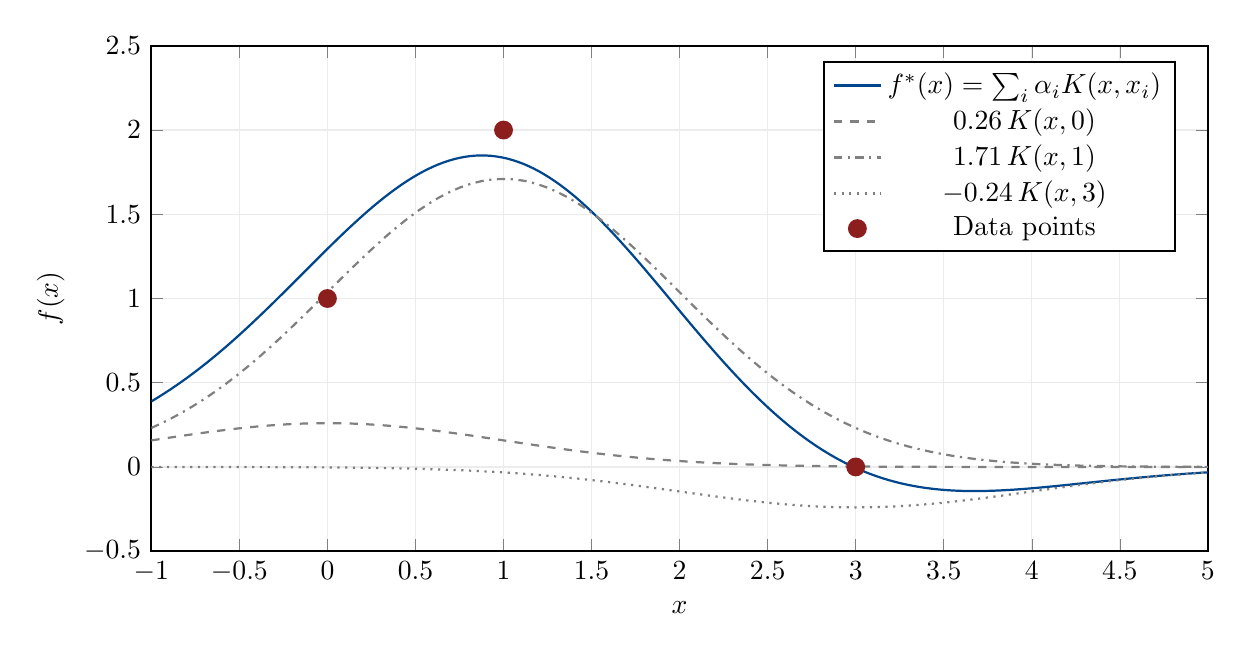
\begin{tikzpicture}
\begin{axis}[
  width=15cm, height=8cm,
  xlabel={$x$}, ylabel={$f(x)$},
  xmin=-1, xmax=5, ymin=-0.5, ymax=2.5,
  legend pos=north east,
  grid=major, grid style={gray!15},
  thick
]
% Gaussian bumps centered at data points
\addplot[defblue, domain=-1:5, samples=200] {0.26*exp(-x^2/2) + 1.71*exp(-(x-1)^2/2) - 0.24*exp(-(x-3)^2/2)};
\addlegendentry{$f^*(x) = \sum_i \alpha_i K(x,x_i)$}

% Individual bumps
\addplot[gray, dashed, domain=-1:5, samples=100] {0.26*exp(-x^2/2)};
\addlegendentry{$0.26\,K(x,0)$}
\addplot[gray, dashdotted, domain=-1:5, samples=100] {1.71*exp(-(x-1)^2/2)};
\addlegendentry{$1.71\,K(x,1)$}
\addplot[gray, dotted, domain=-1:5, samples=100] {-0.24*exp(-(x-3)^2/2)};
\addlegendentry{$-0.24\,K(x,3)$}

% Data points
\addplot[only marks, mark=*, mark size=3pt, thmred] coordinates {(0,1) (1,2) (3,0)};
\addlegendentry{Data points}
\end{axis}
\end{tikzpicture}
\caption{Kernel ridge regression with the Gaussian kernel ($\sigma=1$,
$\lambda=0.1$). The learned function $f^*$ (solid blue) is a weighted
sum of Gaussian bumps centered at the data points. The individual
weighted bumps are shown as dashed/dotted gray curves. The red dots are
the training data $(x_i, y_i)$.}
\label{rkhs:fig:kernel_ridge}
\end{figure}

% ══════════════════════════════════════════════════════════════
\section{Concrete RKHS for Common Kernels}
\label{rkhs:sec:examples_rkhs}
% ══════════════════════════════════════════════════════════════

What do the functions in $\hk$ actually look like for specific kernels?
This section gives concrete characterizations.

% ────────────────────────────
\subsection{Linear Kernel}

For $K(x,x') = x^\top x'$ on $\R^d$:

The canonical feature map
(Definition~\ref{rkhs:def:canonical_feature}) sends each
point $x \in \R^d$ to the linear functional
$K(\cdot, x): z \mapsto z^\top x$. With the
identification $w \leftrightarrow f_w$, where
$f_w(z) = z^\top w$:
\begin{itemize}
  \item The RKHS is
    $\hk = \{f_w : z \mapsto z^\top w \;\mid\;
    w \in \R^d\}$ --- the set of linear functionals
    on $\R^d$.
  \item The RKHS inner product is
    $\inner{f_w}{f_v}_{\hk} = w^\top v$, and the
    RKHS norm is $\norm{f_w}_{\hk} = \norm{w}_2$.
  \item \textbf{Reproducing property check}:
    $\inner{f_w}{K(\cdot,x)}_{\hk}
    = \inner{f_w}{f_x}_{\hk} = w^\top x
    = f_w(x)$. \checkmark
  \item The Representer Theorem says
    $w^* = \sum_i \alpha_i x_i$ (the optimal weight
    vector lies in the span of the data).
\end{itemize}

So kernel ridge regression with the linear kernel recovers ordinary
ridge regression.

% ────────────────────────────
\subsection{Polynomial Kernel}

For $K(x,x') = (x^\top x')^p$ on $\R^d$, the RKHS is
\textbf{finite-dimensional}:
\begin{itemize}
  \item $\hk$ consists of \emph{homogeneous polynomials
    of degree $p$} in $d$ variables. The dimension is
    $\binom{d+p-1}{p}$.
  \item For $p = 2$ in $\R^2$:
    $\hk = \{f(z) = a\,z_1^2 + b\,z_1 z_2 + c\,z_2^2
    : a,b,c \in \R\}$, a $3$-dimensional space.
  \item Since $\hk$ is finite-dimensional, every function
    $f \in \hk$ is uniquely determined by finitely many
    coefficients. The Riesz identification between $f$
    and a coefficient vector in $\R^{\binom{d+p-1}{p}}$
    is exact---this is why the vector notation
    $\phi(x) \in \R^3$ from Example~5 is fully rigorous,
    not merely a shorthand.
  \item The RKHS norm penalizes monomial coefficients
    unevenly: it reflects the inner product geometry
    induced by the kernel (e.g., the $\sqrt{2}$ factor
    on the cross-term in the quadratic case).
\end{itemize}

\textbf{Key contrast with the Gaussian kernel.}
The polynomial RKHS is the only common case where
$\mathcal{F}$ is finite-dimensional, so we can
legitimately write $\phi_x$ as a vector. For the
Gaussian kernel below, the RKHS is
infinite-dimensional and no such vector
representation exists.

% ────────────────────────────
\subsection{Gaussian (RBF) Kernel}

For $K(x,x') = \exp(-\norm{x-x'}^2/2\sigma^2)$ on $\R^d$:
\begin{itemize}
  \item The RKHS is \textbf{infinite-dimensional} and contains very
  smooth functions.
  \item Functions in $\hk$ are infinitely differentiable ($C^\infty$)
  and analytic.
  \item Intuitively, $\hk$ contains functions that can be represented as
  weighted sums of Gaussian ``bumps'' centered at arbitrary locations:
  $f(x) = \int \alpha(t)\,\exp(-\norm{x-t}^2/2\sigma^2)\,dt$.
  \item The RKHS norm penalizes ``roughness'': rapidly oscillating
  functions have large $\norm{f}_{\hk}$.
  \item Smaller $\sigma$ allows finer detail but makes the RKHS norm of
  a given function larger.
\end{itemize}

\begin{insightbox}[The Feature Map of the Gaussian Kernel is
Infinite-Dimensional]
Using the Taylor expansion $e^z = \sum_{k=0}^\infty z^k/k!$ with $z =
x^\top x' / \sigma^2$:
\begin{align*}
K(x,x') &= e^{-\norm{x}^2/2\sigma^2}\; e^{x^\top x'/\sigma^2}\; e^{-\norm{x'}^2/2\sigma^2} \\
&= e^{-\norm{x}^2/2\sigma^2} \sum_{k=0}^\infty \frac{(x^\top x')^k}{k!\,\sigma^{2k}}\; e^{-\norm{x'}^2/2\sigma^2}.
\end{align*}
Each term $(x^\top x')^k$ is a polynomial kernel of degree $k$,
contributing a finite-dimensional feature space. Summing over all $k$
yields an \textbf{infinite-dimensional} feature space.

This means: the Gaussian kernel implicitly includes polynomial features
of \emph{every} degree.
\end{insightbox}

% ══════════════════════════════════════════════════════════════
\section{Summary of Key Relationships}
\label{rkhs:sec:summary}
% ══════════════════════════════════════════════════════════════

The following table summarizes how the key concepts relate to each other:

\begin{center}
\renewcommand{\arraystretch}{1.4}
\begin{tabular}{@{}p{4cm}p{9.5cm}@{}}
\toprule
\textbf{Concept} & \textbf{Role in the RKHS Framework} \\
\midrule
P.D.\ kernel $K$ & Measures similarity; determines the RKHS uniquely
(Moore--Aronszajn) \\
Gram matrix $\mat{K}$ & The $n \times n$ computable matrix of kernel
evaluations at data points \\
Feature map $\phi$ & Maps inputs to a space where $K(x,x') =
\inner{\phi(x)}{\phi(x')}$ \\
RKHS $\hk$ & Hilbert space of functions with the reproducing property \\
RKHS norm $\norm{f}_{\hk}$ & Measures function ``complexity''; used for
regularization \\
Reproducing property & $f(x) = \inner{f}{K(\cdot,x)}$; evaluation =
inner product \\
Representer Theorem & Optimal $f^* = \sum_i \alpha_i K(\cdot, x_i)$;
reduces to finite dimensions \\
Kernelized problem & $\min_{\vect{\alpha}}
\,\mathrm{Loss}(\mat{K}\vect{\alpha}, \mat{y}) +
\lambda\,\vect{\alpha}^\top\mat{K}\vect{\alpha}$ \\
\bottomrule
\end{tabular}
\end{center}

% ══════════════════════════════════════════════════════════════
% \section{Application: Manifold Regularization}
% \label{rkhs:sec:applications}
% % ══════════════════════════════════════════════════════════════

% The RKHS framework becomes particularly powerful in semi-supervised
% learning, where we have few labeled examples but many unlabeled ones
% connected by a graph. \emph{Manifold regularization} combines RKHS
% complexity control with graph smoothness.

% % ────────────────────────────
% \subsection{The Manifold Regularization Objective}

% Suppose we have $n$ data points, of which $l$ are labeled. We construct
% a graph over all $n$ points (e.g., a $k$-nearest-neighbor graph) with
% Laplacian $\mat{L}$.

% \begin{theorembox}[Manifold Regularization (Belkin et al., 2006)]
% \begin{theorem}
% \label{rkhs:thm:manifold_reg}
% Consider the optimization problem:
% \begin{equation}
% \label{rkhs:eq:manifold_reg}
% \min_{f \in \hk}\; \underbrace{\frac{1}{l}\sum_{i=1}^{l} \ell(f(x_i), y_i)}_{\text{supervised loss}} + \underbrace{\gamma_A \norm{f}_{\hk}^2}_{\substack{\text{ambient regularizer:}\\\text{smooth in feature space}}} + \underbrace{\frac{\gamma_I}{n^2}\,\mat{f}^\top \mat{L}\, \mat{f}}_{\substack{\text{intrinsic regularizer:}\\\text{smooth along graph}}}
% \end{equation}
% where $\mat{f} = (f(x_1), \ldots, f(x_n))^\top$ and $\gamma_A, \gamma_I > 0$.

% By an extended Representer Theorem, the minimizer has the form $f^*(x) =
% \sum_{i=1}^n \alpha_i K(x, x_i)$, now involving \textbf{all} $n$ points
% (not just the $l$ labeled ones).
% \end{theorem}
% \end{theorembox}

% % ────────────────────────────
% \subsection{Kernelization}

% Using $\mat{f} = \mat{K}\vect{\alpha}$ and $\norm{f}^2_{\hk} =
% \vect{\alpha}^\top\mat{K}\vect{\alpha}$
% (equation~\eqref{rkhs:eq:rkhs_norm_alpha}):

% \begin{equation}
% \label{rkhs:eq:manifold_kernelized}
% \min_{\vect{\alpha} \in \R^n}\; \frac{1}{l}\sum_{i=1}^{l} \ell\bigl((\mat{K}\vect{\alpha})_i, y_i\bigr) + \gamma_A\,\vect{\alpha}^\top\mat{K}\vect{\alpha} + \frac{\gamma_I}{n^2}\,\vect{\alpha}^\top \mat{K}\mat{L}\mat{K}\vect{\alpha}
% \end{equation}

% This is a finite-dimensional optimization over $\vect{\alpha} \in \R^n$,
% solvable by standard methods.

% \begin{insightbox}[Two Complementary Regularizers]
% The two regularizers encode different types of prior knowledge:

% \textbf{Ambient regularizer} ($\gamma_A\norm{f}_{\hk}^2$): Penalizes
% complexity in the feature space, just like standard SVMs. This prevents
% overfitting to the training data in the ``ambient'' $\R^d$ space.

% \textbf{Intrinsic regularizer} ($\gamma_I\,\mat{f}^\top\mat{L}\mat{f}$):
% Penalizes functions that change rapidly across graph edges. Since
% $\mat{f}^\top\mat{L}\mat{f} = \sum_{(i,j) \in E} w_{ij}(f(x_i) -
% f(x_j))^2$, this forces the learned function to be smooth with respect
% to the \emph{geometry of the data manifold} (captured by the graph).
% Crucially, this term involves \textbf{all} $n$ data points --- both
% labeled and unlabeled --- which is how unlabeled data improves the
% solution.
% \end{insightbox}
% ══════════════════════════════════════════════════════════════
% ══════════════════════════════════════════════════════════════
\section{Application: Manifold Regularization}
\label{rkhs:sec:applications}
% ══════════════════════════════════════════════════════════════

The RKHS framework becomes particularly powerful in 
\textbf{semi-supervised learning}, where we have few labeled
examples but many unlabeled ones. This is the rule, not the
exception, in real-world applications: labeling requires human
effort, but unlabeled data is abundant.

\begin{insightbox}[The Fundamental Challenge]
How can unlabeled data possibly help? If we only have inputs 
$x_1,\ldots,x_n$ without labels, what additional information do 
they provide about the function $f$ we want to learn?

\textbf{Key idea:} The unlabeled data reveal the \emph{geometry} 
of the data distribution. If two points $x_i$ and $x_j$ are 
connected by a high-density path in input space (high-weight edges), 
their predictions $f(x_i)$ and $f(x_j)$ should be similar. This is the 
\textbf{manifold assumption}: data lie near a low-dimensional 
manifold, and the target function varies smoothly along it.
\end{insightbox}

% ────────────────────────────
\subsection{The Manifold Assumption in Pictures}
\label{rkhs:subsec:manifold_intuition}

\begin{figure}[ht]
\centering
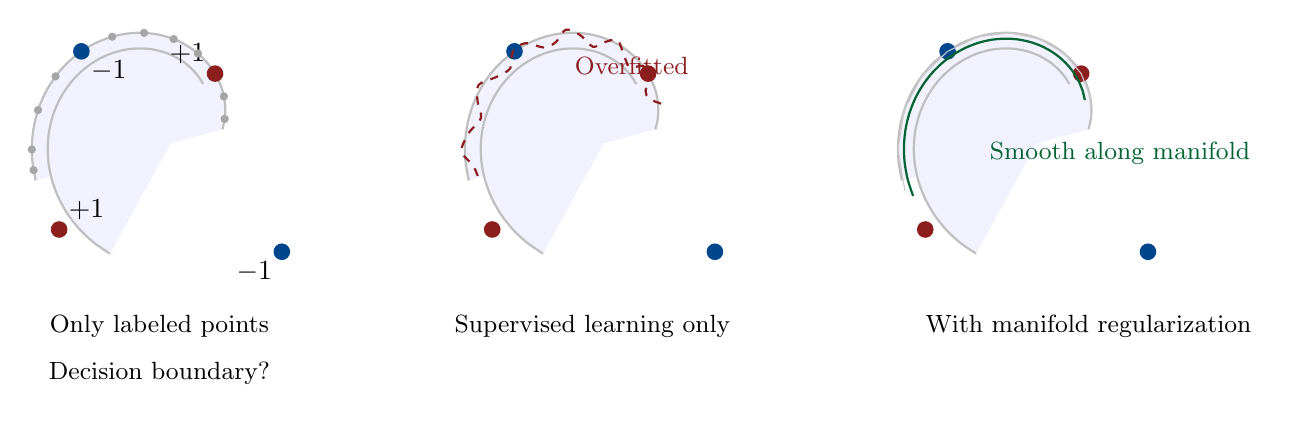
\begin{tikzpicture}[scale=1.0]
% Left: Swiss roll with labeled points only
\begin{scope}[xshift=-4cm]
  \draw[thick, gray!50, fill=blue!5] 
    plot[domain=0:4.5, smooth] 
    ({cos(deg(2*pi*\x/8))*(0.8+0.2*\x)}, 
     {sin(deg(2*pi*\x/8))*(0.8+0.2*\x)});
  \draw[thick, gray!50, fill=blue!5] 
    plot[domain=0:4.5, smooth] 
    ({cos(deg(2*pi*\x/8+0.8))*(0.8+0.2*\x)}, 
     {sin(deg(2*pi*\x/8+0.8))*(0.8+0.2*\x)});
  
  % Labeled points (few)
  \fill[thmred] 
    ({cos(deg(2*pi*1/8))*(0.8+0.2*1)}, 
     {sin(deg(2*pi*1/8))*(0.8+0.2*1)}) 
    circle (3pt) node[above left, black] {$+1$};
  \fill[defblue] 
    ({cos(deg(2*pi*3/8))*(0.8+0.2*3)}, 
     {sin(deg(2*pi*3/8))*(0.8+0.2*3)}) 
    circle (3pt) node[below right, black] {$-1$};
  \fill[thmred] 
    ({cos(deg(2*pi*5/8))*(0.8+0.2*5)}, 
     {sin(deg(2*pi*5/8))*(0.8+0.2*5)}) 
    circle (3pt) node[above right, black] {$+1$};
  \fill[defblue] 
    ({cos(deg(2*pi*7/8))*(0.8+0.2*7)}, 
     {sin(deg(2*pi*7/8))*(0.8+0.2*7)}) 
    circle (3pt) node[below left, black] {$-1$};
  
  % Unlabeled points (many, gray)
  \foreach \t in {0.2,0.6,1.4,1.8,2.2,2.6,3.4,3.8,4.2,4.4} {
    \fill[gray!70] 
      ({cos(deg(2*pi*\t/8))*(0.8+0.2*\t)}, 
       {sin(deg(2*pi*\t/8))*(0.8+0.2*\t)}) 
      circle (1.5pt);
  }
  
  \node[font=\small] at (0, -2.5) {Only labeled points};
  \node[font=\small] at (0, -3.1) {Decision boundary?};
\end{scope}

% Middle: Pure supervised decision boundary
\begin{scope}[xshift=1.5cm]
  \draw[thick, gray!50, fill=blue!5] 
    plot[domain=0:4.5, smooth] 
    ({cos(deg(2*pi*\x/8))*(0.8+0.2*\x)}, 
     {sin(deg(2*pi*\x/8))*(0.8+0.2*\x)});
  \draw[thick, gray!50, fill=blue!5] 
    plot[domain=0:4.5, smooth] 
    ({cos(deg(2*pi*\x/8+0.8))*(0.8+0.2*\x)}, 
     {sin(deg(2*pi*\x/8+0.8))*(0.8+0.2*\x)});
  
  % Same labeled points
  \fill[thmred] 
    ({cos(deg(2*pi*1/8))*(0.8+0.2*1)}, 
     {sin(deg(2*pi*1/8))*(0.8+0.2*1)}) circle (3pt);
  \fill[defblue] 
    ({cos(deg(2*pi*3/8))*(0.8+0.2*3)}, 
     {sin(deg(2*pi*3/8))*(0.8+0.2*3)}) circle (3pt);
  \fill[thmred] 
    ({cos(deg(2*pi*5/8))*(0.8+0.2*5)}, 
     {sin(deg(2*pi*5/8))*(0.8+0.2*5)}) circle (3pt);
  \fill[defblue] 
    ({cos(deg(2*pi*7/8))*(0.8+0.2*7)}, 
     {sin(deg(2*pi*7/8))*(0.8+0.2*7)}) circle (3pt);
  
  % Supervised decision boundary (wiggly, overfitted)
  \draw[thmred, thick, dashed] 
    plot[domain=0.2:4.3, smooth] 
    ({cos(deg(2*pi*\x/8+0.2))*(0.8+0.2*\x+0.1*sin(deg(10*\x)))}, 
     {sin(deg(2*pi*\x/8+0.2))*(0.8+0.2*\x+0.1*sin(deg(10*\x)))});
  \node[font=\small, thmred] at (0.5, 0.8) {Overfitted};
  
  \node[font=\small] at (0, -2.5) {Supervised learning only};
\end{scope}

% Right: Manifold regularization
\begin{scope}[xshift=7cm]
  \draw[thick, gray!50, fill=blue!5] 
    plot[domain=0:4.5, smooth] 
    ({cos(deg(2*pi*\x/8))*(0.8+0.2*\x)}, 
     {sin(deg(2*pi*\x/8))*(0.8+0.2*\x)});
  \draw[thick, gray!50, fill=blue!5] 
    plot[domain=0:4.5, smooth] 
    ({cos(deg(2*pi*\x/8+0.8))*(0.8+0.2*\x)}, 
     {sin(deg(2*pi*\x/8+0.8))*(0.8+0.2*\x)});
  
  % Same labeled points
  \fill[thmred] 
    ({cos(deg(2*pi*1/8))*(0.8+0.2*1)}, 
     {sin(deg(2*pi*1/8))*(0.8+0.2*1)}) circle (3pt);
  \fill[defblue] 
    ({cos(deg(2*pi*3/8))*(0.8+0.2*3)}, 
     {sin(deg(2*pi*3/8))*(0.8+0.2*3)}) circle (3pt);
  \fill[thmred] 
    ({cos(deg(2*pi*5/8))*(0.8+0.2*5)}, 
     {sin(deg(2*pi*5/8))*(0.8+0.2*5)}) circle (3pt);
  \fill[defblue] 
    ({cos(deg(2*pi*7/8))*(0.8+0.2*7)}, 
     {sin(deg(2*pi*7/8))*(0.8+0.2*7)}) circle (3pt);
  
  % Graph edges connecting nearby points along the manifold
  \foreach \t in {0.2,0.6,1.0,1.4,1.8,2.2,2.6,3.0,3.4,3.8,4.2} {
    \pgfmathsetmacro{\next}{\t+0.4}
    \draw[gray!40, thin] 
      ({cos(deg(2*pi*\t/8))*(0.8+0.2*\t)}, 
       {sin(deg(2*pi*\t/8))*(0.8+0.2*\t)}) --
      ({cos(deg(2*pi*\next/8))*(0.8+0.2*\next)}, 
       {sin(deg(2*pi*\next/8))*(0.8+0.2*\next)});
  }
  
  % Manifold-aware decision boundary
  \draw[exgreen, thick] 
    plot[domain=0.2:4.3, smooth] 
    ({cos(deg(2*pi*\x/8+0.3))*(0.8+0.2*\x)}, 
     {sin(deg(2*pi*\x/8+0.3))*(0.8+0.2*\x)});
  \node[font=\small, exgreen] at (1.2, -0.3) {Smooth along manifold};
  
  \node[font=\small] at (0.8, -2.5) {With manifold regularization};
\end{scope}
\end{tikzpicture}
\caption{Why unlabeled data matter. \textbf{Left:} Only four labeled 
points on a Swiss roll manifold. \textbf{Middle:} A pure supervised 
method overfits. \textbf{Right:} Manifold regularization uses graph 
connections (gray edges) to enforce smoothness along the manifold.}
\label{rkhs:fig:manifold_motivation}
\end{figure}

% ────────────────────────────
\subsection{From Graphs to Geometry: The Graph Laplacian}
\label{rkhs:subsec:graph_laplacian}

How do we encode manifold structure mathematically? We build a graph
connecting nearby points.

\begin{definitionbox}[Definition: Graph Laplacian]
\begin{definition}[Graph Laplacian]
\label{rkhs:def:graph_laplacian}
Given $n$ points $x_1,\ldots,x_n \in \X$, construct a 
\textbf{similarity graph}:
\begin{itemize}
  \item \textbf{Nodes:} the $n$ data points
  \item \textbf{Edges:} connect $x_i$ and $x_j$ if they are ``close'' 
    (e.g., $k$-nearest neighbors or $\|x_i - x_j\| < \varepsilon$)
  \item \textbf{Weights:} $w_{ij} = 1$ for unweighted graph, or 
    $w_{ij} = \exp(-\|x_i - x_j\|^2/2\sigma^2)$
\end{itemize}
Define the \textbf{degree} of node $i$ as $d_i = \sum_{j=1}^n w_{ij}$.
Then the \textbf{graph Laplacian} $\mat{L} \in \R^{n \times n}$ is:
\[
\mat{L}_{ij} = 
\begin{cases}
d_i & \text{if } i = j \\
-w_{ij} & \text{if } i \neq j
\end{cases}
\]
Equivalently, $\mat{L} = \mat{D} - \mat{W}$, where $\mat{W}$ is the 
weight matrix and $\mat{D} = \operatorname{diag}(d_1,\ldots,d_n)$.
\end{definition}
\end{definitionbox}

\begin{proposition}[Key Properties of the Graph Laplacian]
\leavevmode
\label{rkhs:prop:laplacian_properties}
\begin{enumerate}[label=(\roman*)]
  \item $\mat{L}$ is symmetric and positive semi-definite.
  \item For any vector $\mat{f} = (f(x_1),\ldots,f(x_n))^\top \in \R^n$:
  \begin{equation}
  \label{rkhs:eq:laplacian_quadratic}
  \mat{f}^\top \mat{L} \mat{f} = \frac{1}{2} \sum_{i,j=1}^n w_{ij} 
    \bigl(f(x_i) - f(x_j)\bigr)^2.
  \end{equation}
  \item The quadratic form measures \textbf{smoothness}: it is small 
    when $f$ varies slowly across edges with large weight $w_{ij}$.
\end{enumerate}
\end{proposition}

\begin{proof}
For (ii), expand:
\begin{align*}
\mat{f}^\top \mat{L} \mat{f} 
&= \sum_{i,j} f(x_i) \mat{L}_{ij} f(x_j) \\
&= \sum_i d_i f(x_i)^2 - \sum_{i,j} w_{ij} f(x_i) f(x_j) \\
&= \frac{1}{2} \sum_{i,j} w_{ij} \bigl(f(x_i)^2 - 2f(x_i)f(x_j) 
   + f(x_j)^2\bigr) \\
&= \frac{1}{2} \sum_{i,j} w_{ij} \bigl(f(x_i) - f(x_j)\bigr)^2.
\end{align*}
Property (i) follows from (ii): $\mat{f}^\top \mat{L} \mat{f} \geq 0$ 
for all $\mat{f}$, so $\mat{L}$ is PSD.
\end{proof}

\begin{figure}[ht]
\centering
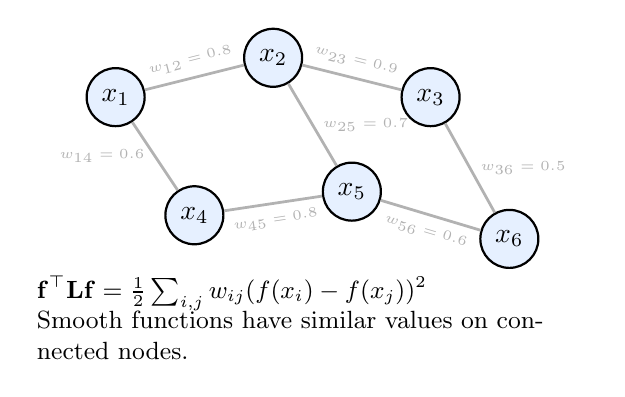
\begin{tikzpicture}[scale=1.0, node distance=1.5cm,
  vertex/.style={circle, draw, fill=lightblue, thick, minimum size=0.7cm},
  edge/.style={gray!60, line width=1.0pt}]

% Graph with 6 nodes
\node[vertex] (v1) at (0,0) {$x_1$};
\node[vertex] (v2) at (2,0.5) {$x_2$};
\node[vertex] (v3) at (4,0) {$x_3$};
\node[vertex] (v4) at (1,-1.5) {$x_4$};
\node[vertex] (v5) at (3,-1.2) {$x_5$};
\node[vertex] (v6) at (5,-1.8) {$x_6$};

% Edges with weights
\draw[edge] (v1) -- node[above, sloped, font=\tiny] {$w_{12}=0.8$} (v2);
\draw[edge] (v2) -- node[above, sloped, font=\tiny] {$w_{23}=0.9$} (v3);
\draw[edge] (v1) -- node[left, font=\tiny] {$w_{14}=0.6$} (v4);
\draw[edge] (v2) -- node[right, font=\tiny] {$w_{25}=0.7$} (v5);
\draw[edge] (v3) -- node[right, font=\tiny] {$w_{36}=0.5$} (v6);
\draw[edge] (v4) -- node[below, sloped, font=\tiny] {$w_{45}=0.8$} (v5);
\draw[edge] (v5) -- node[below, sloped, font=\tiny] {$w_{56}=0.6$} (v6);

% Laplacian quadratic form
\node[font=\small, text width=7cm] at (2.5, -2.8) {
$\mat{f}^\top \mat{L} \mat{f} = \frac{1}{2} \sum_{i,j} w_{ij} 
(f(x_i) - f(x_j))^2$ \\
Smooth functions have similar values on connected nodes.
};
\end{tikzpicture}
\caption{The graph Laplacian encodes manifold geometry. Each edge 
weight $w_{ij}$ measures similarity. The quadratic form penalizes 
differences across edges weighted by similarity.}
\label{rkhs:fig:graph_laplacian}
\end{figure}

% ────────────────────────────
\subsection{The Manifold Regularization Objective}
\label{rkhs:subsec:manifold_objective}

We now combine two sources of information:

\begin{enumerate}[label=\textbf{(\roman*)}]
  \item \textbf{Labeled data:} Supervised loss $\sum_{i=1}^l \ell(f(x_i), y_i)$.
  \item \textbf{Unlabeled data geometry:} Graph smoothness penalty 
    $\mat{f}^\top \mat{L} \mat{f}$.
\end{enumerate}

\begin{theorembox}[Manifold Regularization]
\begin{theorem}[Manifold Regularization]
\label{rkhs:thm:manifold_reg}
Let $\hk$ be an RKHS with kernel $K$, and let $x_1,\ldots,x_n \in \X$ 
be all available data points, of which the first $l$ are labeled with 
targets $y_1,\ldots,y_l \in \R$. Construct a graph over all $n$ points 
with Laplacian $\mat{L}$. Consider:
\begin{equation}
\label{rkhs:eq:manifold_reg}
\min_{f \in \hk}\; \frac{1}{l}\sum_{i=1}^{l} \ell(f(x_i), y_i) 
+ \gamma_A \norm{f}_{\hk}^2 
+ \frac{\gamma_I}{n^2}\,\mat{f}^\top \mat{L}\, \mat{f}
\end{equation}
where $\mat{f} = (f(x_1), \ldots, f(x_n))^\top$ and 
$\gamma_A, \gamma_I > 0$ are regularization parameters.

Then the minimizer admits the following representation:
\begin{equation}
\label{rkhs:eq:manifold_solution}
\boxed{f^*(x) = \sum_{i=1}^n \alpha_i^* K(x, x_i) 
\quad \text{for some } \vect{\alpha}^* \in \R^n}
\end{equation}
\end{theorem}
\end{theorembox}

\begin{insightbox}[Two Regularizers, Two Types of Smoothness]
The two penalty terms encode complementary inductive biases:

\begin{itemize}
  \item \textbf{Ambient regularizer} ($\gamma_A\norm{f}_{\hk}^2$): \\
  Forces $f$ to be smooth in the \emph{ambient space} $\R^d$. This is 
  the standard RKHS penalty from Section~\ref{rkhs:sec:representer}.

  \item \textbf{Intrinsic regularizer} ($\gamma_I \mat{f}^\top \mat{L} \mat{f}$): \\
  Forces $f$ to be smooth along the \emph{data manifold}. Two points 
  connected by a high-weight edge are encouraged to have similar 
  predictions, regardless of their Euclidean distance.
\end{itemize}

The ratio $\gamma_I / \gamma_A$ controls how much we trust the 
unlabeled data geometry versus the supervised signal. When 
$\gamma_I = 0$, we recover standard supervised kernel methods.
\end{insightbox}

% ────────────────────────────
\subsection{Proof of the Extended Representer Theorem}
\label{rkhs:subsec:manifold_representer_proof}

Why does the solution still have the form $\sum_{i=1}^n \alpha_i 
K(\cdot, x_i)$, now using \textbf{all} $n$ points? The proof is an 
elegant extension of the classical Representer Theorem.

\begin{proof}[Proof Sketch]
Let $M = \spn\{K(\cdot, x_1), \ldots, K(\cdot, x_n)\} \subseteq \hk$. 
Any $f \in \hk$ decomposes as $f = f_\parallel + f_\perp$ with 
$f_\parallel \in M$ and $f_\perp \in M^\perp$.

\smallskip
\textbf{Step 1: The loss and intrinsic regularizer see only $f_\parallel$.}
\begin{itemize}
  \item By the reproducing property, $f(x_i) = \inner{f}{K(\cdot, x_i)} 
    = f_\parallel(x_i)$ for each $i = 1,\ldots,n$. Hence the supervised 
    loss depends only on $f_\parallel$.
  \item The vector $\mat{f} = (f(x_1),\ldots,f(x_n))^\top$ is determined 
    entirely by $f_\parallel$, so $\mat{f}^\top \mat{L} \mat{f}$ also 
    depends only on $f_\parallel$.
\end{itemize}

\textbf{Step 2: The ambient regularizer penalizes $f_\perp$ without 
contributing to the other terms.}
By orthogonality, $\norm{f}_{\hk}^2 = \norm{f_\parallel}_{\hk}^2 
+ \norm{f_\perp}_{\hk}^2 \geq \norm{f_\parallel}_{\hk}^2$.

\textbf{Step 3: Conclude.}
For any $f$, the objective $J(f) \geq J(f_\parallel)$ with equality 
iff $f_\perp = 0$. Therefore the minimizer must lie in $M$, i.e., 
$f^* = \sum_{i=1}^n \alpha_i K(\cdot, x_i)$.
\end{proof}

\begin{remark}
The crucial difference from the classical Representer Theorem: the 
intrinsic regularizer involves \emph{evaluations} $f(x_i)$ at 
\textbf{all} $n$ points, not just the labeled ones. This is why the 
expansion now includes \emph{every} data point.
\end{remark}

% ────────────────────────────
\subsection{Kernelization: The Manifold Regularization Algorithm}
\label{rkhs:subsec:manifold_kernelization}

As in Section~\ref{rkhs:sec:representer}, substitute 
$f(x) = \sum_{j=1}^n \alpha_j K(x, x_j)$ into the objective.

\begin{align*}
\text{Prediction vector:} &\quad \mat{f} = \mat{K} \vect{\alpha}, \\
\text{Ambient regularizer:} &\quad \norm{f}_{\hk}^2 
  = \vect{\alpha}^\top \mat{K} \vect{\alpha}, \\
\text{Intrinsic regularizer:} &\quad \mat{f}^\top \mat{L} \mat{f} 
  = \vect{\alpha}^\top \mat{K} \mat{L} \mat{K} \vect{\alpha}.
\end{align*}

\begin{theorembox}[Kernelized Manifold Regularization]
\label{rkhs:thm:manifold_kernelized}
The manifold regularization problem~\eqref{rkhs:eq:manifold_reg} reduces to:
\begin{equation}
\label{rkhs:eq:manifold_kernelized}
\boxed{\min_{\vect{\alpha} \in \R^n}\; 
\frac{1}{l}\sum_{i=1}^{l} \ell\bigl((\mat{K}\vect{\alpha})_i,\; y_i\bigr) 
+ \gamma_A\,\vect{\alpha}^\top\mat{K}\vect{\alpha} 
+ \frac{\gamma_I}{n^2}\,\vect{\alpha}^\top \mat{K}\mat{L}\mat{K}\vect{\alpha}}
\end{equation}
This is convex for convex loss functions $\ell$ (e.g., squared loss, 
hinge loss, logistic loss).
\end{theorembox}

% ────────────────────────────
\subsection{Concrete Example: Two Moons Dataset}
\label{rkhs:subsec:manifold_example}

Let's work through a complete numerical example to see manifold 
regularization in action.

\begin{examplebox}[Example 11: Two Moons Dataset]
\label{rkhs:ex:manifold_two_moons}

\textbf{Setup:} Generate the classic ``two moons'' dataset: 200 points 
in $\R^2$, 100 per class. Label only 4 points (2 per class). Use 196 
unlabeled points to reveal the manifold structure.

\begin{center}
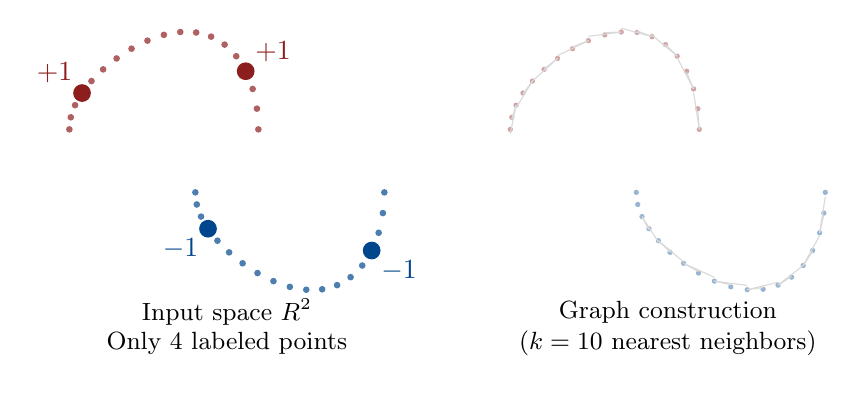
\begin{tikzpicture}[scale=0.8]
% Two moons dataset
\begin{scope}[xshift=-1cm, yshift=-0.5cm]
  % Moon 1 (class +1)
  \foreach \t in {0,10,...,180} {
    \pgfmathsetmacro{\x}{1.5*cos(\t)}
    \pgfmathsetmacro{\y}{1.5*sin(\t) + 0.2*sin(2*\t)}
    \fill[thmred!70] (\x, \y) circle (1.5pt);
  }
  % Moon 2 (class -1)
  \foreach \t in {180,190,...,360} {
    \pgfmathsetmacro{\x}{1.5*cos(\t) + 2}
    \pgfmathsetmacro{\y}{1.5*sin(\t) - 1 + 0.2*sin(2*\t)}
    \fill[defblue!70] (\x, \y) circle (1.5pt);
  }
  
  % Labeled points (only 4!)
  \fill[thmred] ({1.5*cos(30)}, {1.5*sin(30)+0.2*sin(60)}) 
    circle (4pt) node[above right] {$+1$};
  \fill[thmred] ({1.5*cos(150)}, {1.5*sin(150)+0.2*sin(300)}) 
    circle (4pt) node[above left] {$+1$};
  \fill[defblue] ({1.5*cos(210)+2}, {1.5*sin(210)-1+0.2*sin(420)}) 
    circle (4pt) node[below left] {$-1$};
  \fill[defblue] ({1.5*cos(330)+2}, {1.5*sin(330)-1+0.2*sin(660)}) 
    circle (4pt) node[below right] {$-1$};
  
  \node[font=\small] at (1, -2.9) {Input space $\R^2$};
  \node[font=\small] at (1, -3.4) {Only 4 labeled points};
\end{scope}

% Graph construction
\begin{scope}[xshift=6cm, yshift=-0.5cm]
  % Same points, now with edges
  \foreach \t in {0,10,...,180} {
    \pgfmathsetmacro{\x}{1.5*cos(\t)}
    \pgfmathsetmacro{\y}{1.5*sin(\t) + 0.2*sin(2*\t)}
    \fill[thmred!40] (\x, \y) circle (1.2pt);
  }
  \foreach \t in {180,190,...,360} {
    \pgfmathsetmacro{\x}{1.5*cos(\t) + 2}
    \pgfmathsetmacro{\y}{1.5*sin(\t) - 1 + 0.2*sin(2*\t)}
    \fill[defblue!40] (\x, \y) circle (1.2pt);
  }
  
  % Draw some edges to illustrate k-NN graph
  \foreach \i in {0,20,40,60,80,100,120,140,160} {
    \pgfmathsetmacro{\x}{1.5*cos(\i)}
    \pgfmathsetmacro{\y}{1.5*sin(\i) + 0.2*sin(2*\i)}
    \foreach \j in {\i+10,\i+20} {
      \pgfmathsetmacro{\xx}{1.5*cos(\j)}
      \pgfmathsetmacro{\yy}{1.5*sin(\j) + 0.2*sin(2*\j)}
      \draw[gray!30, thin] (\x,\y) -- (\xx,\yy);
    }
  }
  \foreach \i in {200,220,240,260,280,300,320,340} {
    \pgfmathsetmacro{\x}{1.5*cos(\i) + 2}
    \pgfmathsetmacro{\y}{1.5*sin(\i) - 1 + 0.2*sin(2*\i)}
    \foreach \j in {\i+10,\i+20} {
      \pgfmathsetmacro{\xx}{1.5*cos(\j) + 2}
      \pgfmathsetmacro{\yy}{1.5*sin(\j) - 1 + 0.2*sin(2*\j)}
      \draw[gray!30, thin] (\x,\y) -- (\xx,\yy);
    }
  }
  
  \node[font=\small] at (1, -2.9) {Graph construction};
  \node[font=\small] at (1, -3.4) {($k=10$ nearest neighbors)};
\end{scope}
\end{tikzpicture}
\captionof{figure}{Two moons dataset. \textbf{Left:} Only 4 labeled points. 
\textbf{Right:} A $k$-NN graph built from all 200 points reveals the 
two manifold structures.}
\label{rkhs:fig:two_moons_data}
\end{center}

\medskip
\textbf{Algorithm parameters:}
\begin{itemize}
  \item Kernel: Gaussian RBF, $\sigma = 0.5$.
  \item Graph: $k = 10$ NN, Gaussian weights with $\sigma_g = 0.5$.
  \item Regularization: $\gamma_A = 0.01$, $\gamma_I = 1.0$.
  \item Loss: Squared loss $\ell(p,y) = (p - y)^2$.
\end{itemize}

\medskip
\textbf{Step 1: Compute $\mat{K}$ and $\mat{L}$.}
\begin{itemize}
  \item $\mat{K} \in \R^{200 \times 200}$: 
    $K_{ij} = \exp(-\|x_i - x_j\|^2 / 2\sigma^2)$.
  \item $\mat{L} = \mat{D} - \mat{W}$ where 
    $\mat{W}_{ij} = \exp(-\|x_i - x_j\|^2 / 2\sigma_g^2)$ for $k$-NN.
\end{itemize}

\medskip
\textbf{Step 2: Solve for $\vect{\alpha}$.}
For squared loss, problem~\eqref{rkhs:eq:manifold_kernelized} becomes:
\[
\min_{\vect{\alpha}} \frac{1}{l} \|\mat{K}_l \vect{\alpha} - \mat{y}\|^2 
+ \gamma_A \vect{\alpha}^\top \mat{K} \vect{\alpha} 
+ \frac{\gamma_I}{n^2} \vect{\alpha}^\top \mat{K}\mat{L}\mat{K} \vect{\alpha}
\]
where $\mat{K}_l$ is the $l \times n$ submatrix for labeled points.

Taking the gradient gives the linear system:
\[
\left( \frac{1}{l} \mat{K}_l^\top \mat{K}_l + \gamma_A \mat{K} 
+ \frac{\gamma_I}{n^2} \mat{K}\mat{L}\mat{K} \right) \vect{\alpha} 
= \frac{1}{l} \mat{K}_l^\top \mat{y}.
\]

\medskip
\textbf{Step 3: Predict.}
For any test point $x_*$, 
$f^*(x_*) = \sum_{i=1}^n \alpha_i^* K(x_*, x_i)$.

\begin{center}
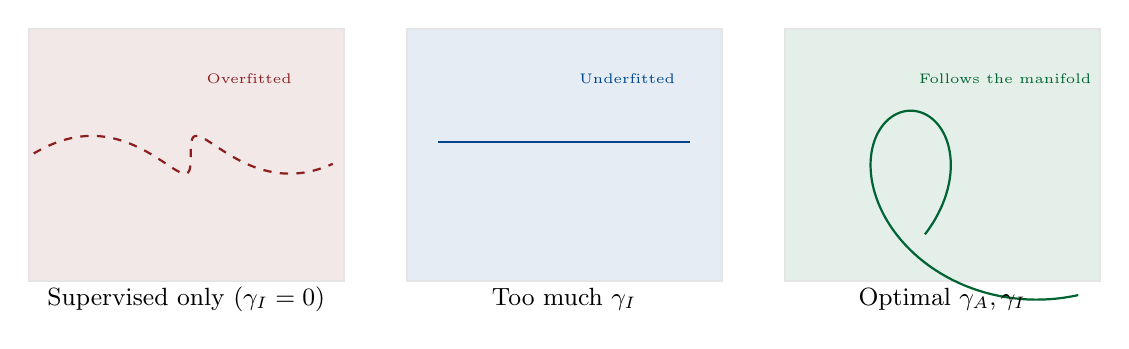
\begin{tikzpicture}[scale=0.8]
% Left: Supervised only
\begin{scope}[xshift=0cm]
  \draw[thick, gray!20, fill=thmred!10] (-1, -2) rectangle (4, 2);
  \draw[thmred, thick, dashed] 
    plot[domain=-0.5:3.5, samples=100] 
    ({0.5*sin(deg(2*\x)) + \x}, {0.3*cos(deg(3*\x))});
  \node[font=\small] at (1.5, -2.3) {Supervised only ($\gamma_I = 0$)};
  \node[font=\tiny, thmred] at (2.5, 1.2) {Overfitted};
\end{scope}
% Middle: Too much graph regularization
\begin{scope}[xshift=6cm]
  \draw[thick, gray!20, fill=defblue!10] (-1, -2) rectangle (4, 2);
  \draw[defblue, thick] (-0.5, 0.2) -- (3.5, 0.2);
  \node[font=\small] at (1.5, -2.3) {Too much $\gamma_I$};
  \node[font=\tiny, defblue] at (2.5, 1.2) {Underfitted};
\end{scope}
% Right: Correct balance
\begin{scope}[xshift=12cm]
  \draw[thick, gray!20, fill=exgreen!10] (-1, -2) rectangle (4, 2);
  \draw[exgreen, thick] 
    plot[domain=-0.2:3.2, samples=100] 
    ({1.5*cos(deg(pi*\x/2)) + \x}, 
     {1.5*sin(deg(pi*\x/2)) - 0.8});
  \node[font=\small] at (1.5, -2.3) {Optimal $\gamma_A, \gamma_I$};
  \node[font=\tiny, exgreen] at (2.5, 1.2) {Follows the manifold};
\end{scope}
\end{tikzpicture}
\captionof{figure}{Effect of the intrinsic regularizer.
\textbf{Left:} Without manifold regularization, overfitting.
\textbf{Middle:} Excessive $\gamma_I$, underfitting.
\textbf{Right:} Properly tuned, the boundary follows the manifold.}
\label{rkhs:fig:manifold_regularization_effect}
\end{center}

\medskip
\textbf{Key takeaway:} With only 4 labeled points, pure supervised 
learning fails. Manifold regularization leverages the 196 unlabeled 
points to produce a decision boundary that respects the true data 
geometry.
\end{examplebox}

% ────────────────────────────
\subsection{Practical Considerations}
\label{rkhs:subsec:manifold_practical}

\begin{enumerate}[label=\textbf{\arabic*.}]
  \item \textbf{Choosing the graph.} 
  \begin{itemize}
    \item $k$-NN graph: common choices $k = 5$--$20$. 
    \item $\varepsilon$-ball graph: connect points within distance $\varepsilon$.
    \item Edge weights: binary, Gaussian, or cosine similarity.
  \end{itemize}
  
  \item \textbf{Normalization.} The factor $1/n^2$ ensures consistent 
    scaling as $n$ grows. Often $\mat{L}$ is replaced by the normalized 
    Laplacian $\mat{L}_{\text{norm}} = \mat{I} - \mat{D}^{-1/2}\mat{W}
    \mat{D}^{-1/2}$.
  
  \item \textbf{Computational cost.} 
  \begin{itemize}
    \item Computing $\mat{K}$ is $O(n^2 d)$, constructing $k$-NN graph 
      is $O(n^2 d)$.
    \item Solving the linear system is $O(n^3)$ — the main bottleneck.
    \item For large $n$, use Nystr\"om approximation or iterative solvers.
  \end{itemize}
  
  \item \textbf{Relation to other methods.}
  \begin{itemize}
    \item \textbf{Laplacian SVM/Laplacian Ridge Regression:} manifold 
      regularization applied to SVMs and kernel ridge regression.
    \item \textbf{Graph neural networks:} modern deep learning analogue.
  \end{itemize}
\end{enumerate}

% ────────────────────────────
\subsection{Connection to Mercer's Theorem}
\label{rkhs:subsec:manifold_mercer}

The two regularizers can be understood through Mercer's theorem:

\begin{itemize}
  \item The \textbf{ambient regularizer} $\gamma_A \norm{f}_{\hk}^2 
    = \gamma_A \sum_k a_k^2/\lambda_k$ penalizes high-frequency 
    components in the eigenbasis of $K$.
  \item The \textbf{intrinsic regularizer} $\gamma_I \mat{f}^\top 
    \mat{L} \mat{f}$ penalizes variations along the data manifold.
\end{itemize}

When the kernel $K$ is aligned with the manifold (e.g., the heat kernel),
these two regularizers become complementary views of the same geometry.

% ────────────────────────────
\subsection{Summary: Why Manifold Regularization Works}
\label{rkhs:subsec:manifold_summary}

\begin{insightbox}[The Manifold Regularization Recipe]
\begin{enumerate}
  \item \textbf{Start with a kernel} $K$ that encodes ambient smoothness.
  \item \textbf{Build a graph} from \emph{all} data points to capture 
    manifold geometry.
  \item \textbf{Add the graph Laplacian penalty} $\mat{f}^\top \mat{L} 
    \mat{f}$ to enforce smoothness along the manifold.
  \item \textbf{Solve} the kernelized problem ($\vect{\alpha} \in \R^n$).
  \item \textbf{Predict} using $f(x) = \sum_{i=1}^n \alpha_i K(x, x_i)$.
\end{enumerate}

The magic: unlabeled data enter through:
\begin{enumerate}[label=(\alph*)]
  \item The representation $f(x) = \sum_{i=1}^n \alpha_i K(x, x_i)$ 
    includes \textbf{all} points.
  \item The graph Laplacian $\mat{L}$ is constructed from \textbf{all} 
    points.
\end{enumerate}
\end{insightbox}

\begin{remark}[Further Reading]
Key references:
\begin{itemize}
  \item Belkin, Niyogi, Sindhwani (2006). ``Manifold Regularization.'' 
    \emph{Journal of Machine Learning Research}.
  \item Zhu (2005). ``Semi-Supervised Learning with Graphs.'' 
    PhD thesis, CMU.
  \item Chapelle, Sch\"olkopf, Zien (2006). 
    \emph{Semi-Supervised Learning}. MIT Press.
\end{itemize}
\end{remark}
% ══════════════════════════════════════════════════════════════
% ══════════════════════════════════════════════════════════════
\newpage
\section{Appendix: Mercer's Theorem (Spectral Characterization)}
\label{rkhs:sec:mercer}
% ══════════════════════════════════════════════════════════════

For continuous kernels on compact domains, Mercer's theorem provides a
spectral decomposition that connects the kernel to the RKHS in an
illuminating way.

\begin{theorembox}[Mercer's Theorem]
\begin{theorem}[Mercer's Theorem]
\label{rkhs:thm:mercer}
Let $\X$ be a compact subset of $\R^d$ and $K: \X \times \X \to \R$ a
continuous positive definite kernel. Then there exist eigenvalues
$\lambda_1 \geq \lambda_2 \geq \cdots \geq 0$ and orthonormal
eigenfunctions $\{e_k\}_{k=1}^\infty \subset L^2(\X)$ such that:
\begin{equation}
\label{rkhs:eq:mercer}
K(x,x') = \sum_{k=1}^\infty \lambda_k\, e_k(x)\, e_k(x'),
\end{equation}
where the convergence is absolute and uniform.
\end{theorem}
\end{theorembox}

\textbf{Connection to the RKHS.} Mercer's theorem reveals that:
\begin{itemize}
  \item The \emph{feature map} is $\phi(x) =
  \bigl(\sqrt{\lambda_1}\,e_1(x),\; \sqrt{\lambda_2}\,e_2(x),\;
  \ldots\bigr) \in \ell^2$.
  \item The RKHS consists of functions $f = \sum_k a_k e_k$ with finite
  RKHS norm:
  \begin{equation}
  \norm{f}_{\hk}^2 = \sum_{k=1}^\infty \frac{a_k^2}{\lambda_k} < \infty.
  \end{equation}
  \item Functions whose expansion coefficients $a_k$ decay faster than
  $\sqrt{\lambda_k}$ belong to the RKHS; those that don't, don't.
  \item Larger eigenvalues $\lambda_k$ correspond to ``easier''
  directions: components along these eigenfunctions are penalized less
  by the RKHS norm.
\end{itemize}

\begin{examplebox}[Example 11: Mercer Expansion of the Gaussian Kernel
on {$[0,1]$}]
For the Gaussian kernel on $[0,1]$, the eigenvalues decay exponentially:
$\lambda_k \sim C\,e^{-c k}$ (the exact form involves Hermite
functions). This rapid decay means:

\begin{enumerate}
  \item The Gaussian RKHS contains only very smooth functions (because
  high-frequency components $e_k$ for large $k$ are heavily penalized by
  $1/\lambda_k$).
  \item A good finite-dimensional approximation is possible: keeping the
  first $K$ eigenfunctions captures most of the kernel's ``energy.''
\end{enumerate}
\end{examplebox}

\begin{insightbox}[Mercer's Theorem Demystifies the RKHS Norm]
The RKHS norm $\norm{f}_{\hk}^2 = \sum_k a_k^2/\lambda_k$ has a
transparent interpretation:
\begin{itemize}
  \item Components along eigenfunctions with \textbf{large} $\lambda_k$
  are penalized \textbf{less} (they correspond to ``smooth'' or
  ``low-frequency'' directions that the kernel ``likes'').
  \item Components along eigenfunctions with \textbf{small} $\lambda_k$
  are penalized \textbf{heavily} (they correspond to ``rough'' or
  ``high-frequency'' directions).
\end{itemize}
So $\norm{f}_{\hk}$ measures the ``roughness'' of $f$ relative to the
smoothness scale defined by $K$.
\end{insightbox}
%
\begin{figure}[h]
\centering
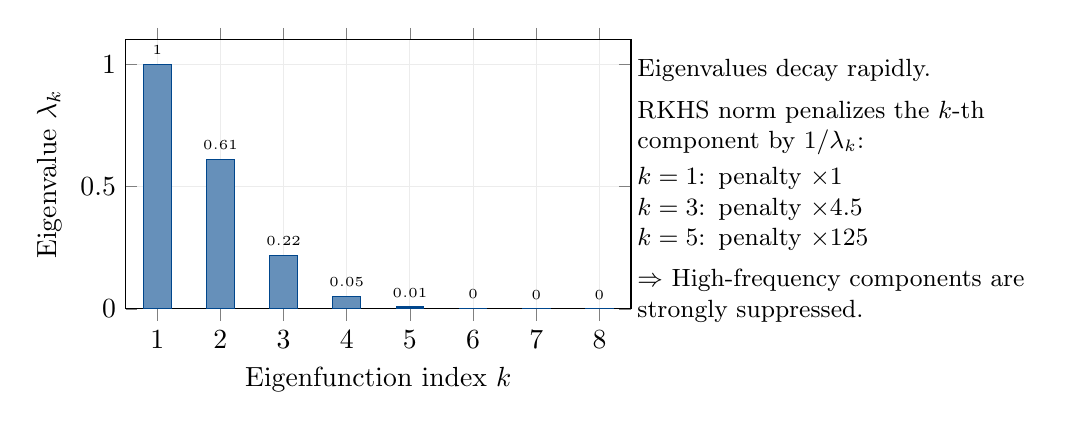
\begin{tikzpicture}[scale=1]
  % Eigenvalue bars
  \begin{axis}[
    width=8cm, height=5cm,
    ybar, bar width=10pt,
    xlabel={Eigenfunction index $k$},
    ylabel={Eigenvalue $\lambda_k$},
    xmin=0.5, xmax=8.5,
    ymin=0, ymax=1.1,
    xtick={1,2,3,4,5,6,7,8},
    grid=major, grid style={gray!15},
    nodes near coords={\pgfmathprintnumber[fixed,precision=2]{\pgfplotspointmeta}},
    every node near coord/.append style={font=\tiny, above},
  ]
  \addplot[fill=defblue!60, draw=defblue] coordinates {
    (1, 1.0) (2, 0.61) (3, 0.22) (4, 0.05) (5, 0.008) (6, 0.001) (7, 0.0001) (8, 0.00001)
  };
  \end{axis}

  % Annotation
  \begin{scope}[xshift=9cm, yshift=1.5cm]
    \node[text width=5cm, font=\small] at (0,0) {
      Eigenvalues decay rapidly.\\[4pt]
      RKHS norm penalizes the $k$-th component by $1/\lambda_k$:\\[2pt]
      $k = 1$: penalty $\times 1$\\
      $k = 3$: penalty $\times 4.5$\\
      $k = 5$: penalty $\times 125$\\[4pt]
      $\Rightarrow$ High-frequency components are strongly suppressed.
    };
  \end{scope}
\end{tikzpicture}
\caption{Schematic eigenvalue spectrum for the Gaussian kernel. The
rapid decay of $\lambda_k$ means the RKHS norm heavily penalizes
high-frequency components, enforcing smoothness.}
\label{rkhs:fig:mercer_eigenvalues}
\end{figure}

% ══════════════════════════════════════════════════════════════
\section{Frequently Asked Questions}
\label{rkhs:sec:faq}
% ══════════════════════════════════════════════════════════════

\begin{enumerate}[label=\textbf{Q\arabic*.}, leftmargin=*, itemsep=10pt]

\item \textbf{Is every Hilbert space of functions an RKHS?}

No. A Hilbert space of functions is an RKHS if and only
if point evaluation is a continuous linear functional
(Proposition~\ref{rkhs:prop:eval_continuous}). In $L^2$,
elements are equivalence classes of functions that
agree almost everywhere, so two ``different'' functions
can represent the same $L^2$ element --- evaluation at
a single point depends on which representative you
choose (see the discussion in
Section~\ref{rkhs:sec:reproducing_property}).

\item \textbf{Is the RKHS unique for a given kernel?}

Yes. The Moore--Aronszajn theorem (Theorem~\ref{rkhs:thm:moore_aronszajn})
guarantees that each p.d.\ kernel determines exactly one RKHS. Different
kernels $\neq$ different RKHS.

\item \textbf{What if I don't regularize ($\lambda = 0$)?}

Without regularization, we minimize only the loss. If the RKHS is rich
(e.g., Gaussian kernel), we can interpolate any data perfectly, but the
solution may be wildly oscillatory (overfitting). The RKHS norm
regularizer $\lambda\norm{f}_{\hk}^2$ prevents this by penalizing
complexity.

\item \textbf{How do I choose the kernel?}

The kernel encodes a prior belief about the function's properties. The
Gaussian kernel assumes smoothness (appropriate for most continuous
data). Polynomial kernels assume the function is polynomial. In
practice, the kernel and its hyperparameters (e.g., $\sigma$) are chosen
via cross-validation.

\item \textbf{How does the RKHS relate to Gaussian Processes?}

A Gaussian Process (GP) with covariance function $K$ is closely related
to the RKHS $\hk$: the RKHS is the set of functions ``supported'' by the
GP (more precisely, the RKHS is the set of mean functions of the
posterior GP). The RKHS norm of $f$ is related to the log-likelihood
under the GP prior.

\item \textbf{Can the RKHS be finite-dimensional?}

Yes --- for the linear kernel $K(x,x') = x^\top x'$, the RKHS is
$d$-dimensional (the set of linear functions). For polynomial kernels of
degree $p$ in $\R^d$, the dimension is $\binom{d+p}{p}$. Only for
kernels like the Gaussian (with infinitely many nonzero Mercer
eigenvalues) is the RKHS infinite-dimensional.

\end{enumerate}

% ══════════════════════════════════════════════════════════════
\section{Conclusion}
\label{rkhs:sec:conclusion}
% ══════════════════════════════════════════════════════════════

The RKHS framework provides an elegant solution to the problem of
learning from data:

\begin{enumerate}[label=\textbf{\arabic*.}]
  \item Start with a \textbf{kernel} $K$ that encodes your prior belief
  about the function's smoothness.
  \item The kernel generates a \textbf{Hilbert space} $\hk$ of candidate
  functions, equipped with a norm that measures complexity.
  \item The \textbf{reproducing property} ensures that evaluation at
  data points is well-behaved.
  \item The \textbf{Representer Theorem} guarantees that the optimal
  regularized function $f^*$ is a finite linear combination of kernel
  evaluations at data points.
  \item Everything reduces to computing with the $n \times n$
  \textbf{Gram matrix} $\mat{K}$.
\end{enumerate}

This framework underlies Support Vector Machines, kernel ridge
regression, Gaussian Processes, and --- when combined with graph
Laplacians --- semi-supervised methods like manifold regularization. The
mathematical beauty is that we get to search over infinite-dimensional
function spaces while only ever solving finite-dimensional optimization
problems.
\end{notechapter}
